% Chapter 3

\chapter{A Convex Formulation for Multi-Task Learning} % Write in your own chapter title
\label{Chapter4}
\lhead{Chapter \ref{Chapter4}. 
\emph{A Convex Formulation for Multi-Task Learning}} % Write in your own chapter title to set the page header

{\bf \small{

}}

\section{Introduction}
% Multi-Task Learning paradigms can be divided in: Feature-Based, Parameter-Based, Joint-Learning
As we have seen in Chapter~\ref{Chapter3}, the MTL proposals can be categorized in feature-based, parameter-based and combination-based approaches. Feature-based proposals have the strategy of finding a shared representation of the original features that is benefitial for all tasks. Parameter-based strategies typically use multi-task regularization schemes that, using specific regularizers, push together the parameters of the task-specialized models.
Finally, the combination-based strategies combine a common model and a task-specific one. 
%
In this chapter we will present a convex formulation for combination-based MTL. With this formulation, a general task-specialized model is defined as
\begin{equation}
    \label{eq:convexmtl_general}
    \begin{aligned}
        h_r(x_i^r)
       = \lambda_r g(x_i^r) + (1 - \lambda_r) g_r(x_i^r) .
    \end{aligned}    
\end{equation}
Here, we use the hyperparameters $\lambda_r \in [0, 1]$ to combine in a convex way the common and specific parts. This general formulation is very flexible, because we can use any family of functions to model $g(\cdot)$ or $g_r(\cdot)$. It is also easily interpretable, since $\lambda_r=1$ for all $r=1, \ldots, \ntasks$ results in a common model and $\lambda_r=0$ in independent models for each task. All the values $\lambda_r \in (0, 1)$ correspond to MTL models, being more common when $\lambda_r$ is close to $1$ and more specific when $\lambda_r$ is close to $0$.
%
Given a MTL sample 
$$\bsample = \bigcup_{r=1}^\ntasks \{(x_1^r, y_1^r), \ldots, (x_{\npertask}^r, y_{\npertask}^r)\},$$
the MTL regularized risk functional that corresponds to this convex formulation is 
\begin{equation}
    \label{eq:convexmtl_general_regrisk}
    \risk_{\bsample} ({g, g_1, \ldots, g_\ntasks}) \defeq \sum_{r=1}^{\ntasks} \sum_{i=1}^{\npertask_r} \lossf(\lambda_r g(x_i^r) + (1 - \lambda_r) g_r(x_i^r), y_i^r) + \mu \left(\Sigma(g) + \sum_{r=1}^\ntasks \Sigma_r(g_r)\right) ,
\end{equation}
where $\Sigma(g)$ and $\Sigma_r(g_r)$ are the regularizers for the common and $r$-th task parts, respectively. Observe that, since the regularization is made independently for each part, no multi-task specific regularization scheme is needed. The task coupling is made directly in the definition of the model, which combines common and specific part, and the risk $\risk_{\bsample}$ is optimized jointly in all parts.
This has some advantages, like the preservation of convexity in the risk minimization problem or an optimization procedure that requires only slight modifications to the standard one, we will see these characteristics in specific applications of this MTL formulation.
%
In this chapter we will show how this formulation can be applied to two of the most popular model families: kernel methods and neural networks; and we will also show how pre-trained models can be convexly combined for MTL.



\section{Convex Multi-Task Learning with Kernel Models}
% Kernel Models are powerful: Kernel trick, high dimensionality representation
As explained in the previous chapters, kernel models offer many good properties such as an implicit transformation to a possibly infinite-dimensional space and the convexity problems that have to be solved in the training process. With these models a regularized risk problem is solved.
% General formulation for a kernel model
A general formulation of training problem for kernel models is 
\begin{equation}
    \label{eq:regrisk_kernel}
    \emprisk({w}) \defeq \sum_{i=1}^{\nsamples} \lossf({w}^\intercal {\phi(\fv{x}_i)} + b, y_i) + \mu \Omega({w}) ,
\end{equation}
where $\sample$ is the sample $\{(x_1, y_1), \ldots, (x_\nsamples, y_\nsamples)\}$ and $\Omega(w)$ is a regularizer for ${w}$, typically the $L_2$ norm: $\norm{w}^2$. Observe that $b$, the bias term, is not regularized since it does not affect the capacity of the hypothesis space.
In~\eqref{eq:regrisk_kernel} $\phi$ is a fixed transformation function such that there exists a ``kernel trick'', that is a kernel function $k$ for which
\begin{equation}
    \nonumber
    \dotp{\phi(x)}{\phi(y)} = k(x, y).
\end{equation}
That is, $\phi$ is an element of \acrshort{rkhs}, where $k$ is the reproducing kernel. 
The Representer Theorem~\citep*{ScholkopfHS01} states that the optimal solution of problem~\eqref{eq:regrisk_kernel} has the following form
\begin{equation}
    \nonumber
    w^* = \sum_{i=1}^\nsamples \alpha_i \phi(x_i)
\end{equation}
where $\alpha_i \in \reals$ are some coefficients. This means that our optimal solution $w^*$ is also an element of the same \acrshort{rkhs}.
These models embrace the Structural Risk Minimization paradigm by limiting the capacity of the space of hypothesis, which is done by penalizing the $L_2$ norm of $w$. This is equivalent to limiting our space of candidates to vectors inside a ball of some fixed radius.

% One of the first multi-task learning approach with kernel models is Regularized MTL
Multi-Task Learning with kernel models require imposing some kind of coupling between the models for each task in the learning process. The feature learning or feature sharing approach, which is usually adopted with neural networks, is not feasible when using kernel models, since the (implicit) transformation functions $\phi$ used are not learned but fixed, and determined by the choice of kernel function. Therefore, other strategies have to be developed. 
One approach to MTL with kernel models was developed in~\cite{EvgeniouP04}, and later extended in~\citet{CaiC09, CaiC12}, where the models for each task are defined as:
\begin{equation}
    \nonumber
    {w}_r = {w} + {v}_r,
\end{equation} 
where $w$ is a common part, shared by all models, and $v_r$ is a task-specific part. With this approximation, the transfer of information is performed by the common part ${w}$.
The regularized risk that is minimized is 
\begin{equation}
    \label{eq:additive_regrisk}
    \risk_{\bsample} ({w, v_1, \ldots, v_\ntasks}) \defeq \sum_{r=1}^{\ntasks} \sum_{i=1}^{\npertask_r} \lossf({w}^\intercal {\phi(\fv{x}_i^r)} + {v}_r^\intercal {\phi_r(\fv{x}_i^r)} + b_r, y_i^r) + \mu_c \norm{{w}}^2 + \mu_s \sum_{r=1}^\ntasks \norm{{v}_r}^2,
\end{equation}
where $\mu_c$ and $\mu_s$ are the hyperparameters to control the common and specific parts regularization, respectively. Here $\bsample$ is an \acrshort{mtl} sample $$\bsample = \bigcup_{r=1}^\ntasks \{(x_1^r, y_1^r), \ldots, (x_{\npertask}^r, y_{\npertask}^r)\}.$$
Observe also that in~\eqref{eq:additive_regrisk} different transformations are used: the transformation $\phi$ corresponds to common part of the model, while $\phi_r$ is task-specific.
%
This is a joint learning approach that is developed for the L1-SVM, to which Evgeniou et al. give the name of \emph{Regularized MTL}, but we will refer to it as {additive} approach.
%
Observe that as $\frac{\mu_c}{\mu_s} \tendsto{}{\infty} $ we would have a common part ${w}$ that tends to zero, which would results in independent models for each task, i.e. ${w}_r \eqsim {v}_r$. On the contrary, when $\frac{\mu_c}{\mu_s} \tendsto{}{0} $, the task-specific parts tend to zero and every model is the common part, i.e. ${w}_r \eqsim {w}$.
There are two asymptotical behaviours: the first one tends to an ITL approach, while the second one tends to a CTL one. The MTL formulation is one strategy that lies between those two approaches, CTL and ITL, combining them to achieve a more flexible model.

% General formulation for a convex MTL Kernel 
The asymptotical properties of this approach offer an interpretation to understand the influence of each hyperparameter, but they are not applicable in practice.
In~\cite{RuizAD19} we propose an alternative formulation for this joint learning approach. The models for each task are defined as a convex combination of the common and task specific parts:
\begin{equation}
    \nonumber
    {w}_r = \lambda {w} + (1 - \lambda) {v}_r,
\end{equation}
where $\lambda \in \left[0, 1\right]$ is a hyperparameter.
More specifically, and using the formulation of~\eqref{eq:convexmtl_general}, we define the common part as $g(x) =  {w}^\intercal {\phi(x)} + b$ and the task-specific parts as $g_r(x) = {v_r}^\intercal {\phi_r(x)} + b_r$, so the MTL models are
\begin{equation}
    \nonumber
    h_r(x_i^r) = \lambda \left\lbrace {w}^\intercal {\phi(x_i^r)} + b \right\rbrace + (1 - \lambda) \left\lbrace {v}_r^\intercal {\phi_r(x_i^r)} + b_r \right\rbrace ,
\end{equation}
and the corresponding regularized risk is 
\begin{equation}
    \nonumber
    \begin{aligned}
        \risk_{\bsample} ({w, v_1, \ldots, v_\ntasks}) \defeq &\sum_{r=1}^{\ntasks} \sum_{i=1}^{\npertask_r} \lossf(\lambda \left\lbrace {w}^\intercal {\phi(x_i^r)} + b \right\rbrace + (1 - \lambda) \left\lbrace {v}_r^\intercal {\phi_r(x_i^r)} + b_r \right\rbrace, y_i^r) \\ 
        &\qquad + \mu_c \norm{{w}}^2 + \mu_s \sum_{r=1}^\ntasks \norm{{v}_r}^2 .
    \end{aligned}
\end{equation}
We will name this approach {convex}, in contrast to the {additive} approach of the original formulation.
% Discussion?
With this formulation, the interpretation of $\lambda$ is straight-forward. The model with $\lambda = 1$ is equivalent to learning a single common model for all tasks, that is ${w}_r = {w}$. When $\lambda=0$, the models for each task are completely independent: ${w}_r = {v}_r$.
The convex formulation also define an MTL model that is between a CTL approach and an ITL one, but it presents two advantages: the values of $\lambda$ that recover the CTL and ITL approaches are known, and these values are specific, not an asymptotical behaviour as in the original formulation. 
%
Moreover, it is shown in the paper that the two formulations, the {additive} and {convex}, are equivalent with an L1-SVM setting.
%
The proposal of~\cite{RuizAD19} is made for L1-SVM, but it is extended to L2 and LS-SVMs in~\cite{RuizAD21}. In this chapter we present the convex formulation for L1, L2 and LS-SVM, as well as the equivalence results between the {additive} and {convex} formulations.




\subsection{L1 Support Vector Machine}
The L1-SVM~\cite{Vapnik00} is the original and most popular variant of the SVMs and is also the basis of the MTL formulation in~\cite{EvgeniouP04}.
I will present the development for the {additive} approach and the one for the {convex} using an L1-SVM setting. Then I will show the equivalence between the two approaches and discuss its differences.

\subsubsection{{Additive} MTL L1-SVM}
% Additive Approach
%   Primal
The {additive} MTL primal problem formulation, presented in~\cite{EvgeniouP04} 
and extended for task-specific biases in~\cite{CaiC12}, is
\begin{equation}\label{eq:svmmtl_primal_add}
    \begin{aligned}
    & \argmin_{w, {v}_r, \xi}
    & & {J({w}, {v}_r, \xi) = C \sum_{r= 1}^T \sum_{i=1}^{m_r} {\xi_{i}^r} + \frac{1}{2} \sum_{r= 1}^T{\norm{{v}_r}^2} + \frac{\mu}{2} {\norm{{w}}}^2} \\
    & \text{s.t.}
    & & y_{i}^r ({w} \cdot \phi(x_{i}^r) + b  + {v}_r \cdot \phi_r(x_{i}^r) + b_r) \geq p_{i}^r - \xi_{i}^r ,  \\
    & & & \xi_{i}^r \geq 0; \;  i=1 , \dotsc , m_r, \;  r= 1,\dotsc, T  . \\
    \end{aligned}
\end{equation}
The prediction model is then 
\begin{equation}
    \nonumber
    h_r(\fv{x}) = {w} \cdot \phi(x_{i}^r) + b  + {v}_r \cdot \phi_r(x_{i}^r) + b_r
\end{equation}
for regression and 
\begin{equation}
    \nonumber
    h_r(\fv{x}) = \sign{ \left({w} \cdot \phi(x_{i}^r) + b  + {v}_r \cdot \phi_r(x_{i}^r) + b_r \right)}
\end{equation}
for classification.
Observe again that the transformation $\phi$ is used for the common part and is shared by all tasks, while the transformation $\phi_r$ is task-specific.

%
In~\eqref{eq:svmmtl_primal_add} there are two kind of hyperparameters: $C$ and $\mu$, which, in combination, balance the different parts of the objective function. 
%
Hyperparameter $C$ plays the same role than in the standard L1-SVM : it balances the tradeoff between the loss incurred by the model, represented by the hinge variables $\xi_i^r$ and complexity of the models, represented by the norms $\norm{{w}}$ and $\norm{{v}_r}$. Large values of $C$ highly penalize the loss, so the resulting models are more complex because they have to adapt to the training sample distribution, but these models generalize worse. Small values of $C$ penalize more the norms of $w$ and $v_r$ so the resulting models are simpler but not so dependent on the training sample.

%
Hyperparameter $\mu$, in combination with $C$, balances the specifity of our models. 
Large values of $\mu$, penalize the common part, resulting in more specific models; while small values of $\mu$, alongside large values of $C$, result in a vanishing regularization of the specific parts which leads to common models.
We can find the following cases:
\begin{itemize}
    \item Reduction to an ITL approach:
    $$\mu \tendsto{}{\infty} \implies h_r(\hat{x}) = {v}_r \cdot \phi_r(\hat{x}) + b_r .$$
    That is, the models are learned independently because the common part vanishes.
    \item Reduction to a CTL approach (with task-specific biases): 
    $$C \tendsto{}{0}, \mu \tendsto{}{0} \implies h_r(\hat{x}) = {w} \cdot \phi(\hat{x}) + b_r .$$
    That is, the model for all tasks is common because the specific parts disappear.
    \item Pure MTL approach:
    $$ \mu_\text{inf} < \mu < \mu_\text{sup} \implies h_r(\hat{x}) =({w} \cdot \phi(\hat{x}) ) + ({v}_r \cdot \phi_r(\hat{x})) + b_r .$$
    There is a range of $\mu$, which is unknown, in which the models combine a common and task-specific part.
\end{itemize}
%   Lagrangian/KKT

Observe that~\eqref{eq:svmmtl_primal_add} is a convex problem. As in the standard case of the L1-SVM, the corresponding dual problem is solved. To obtain the dual problem, it is necessary to express the Lagrangian of problem~\eqref{eq:svmmtl_primal_add}:
\begin{equation}\label{eq:svmmtl_lagrangian_add}
    \begin{aligned}
        & \lagr({w}, \fv{v}_1, \ldots, \fv{v}_\ntasks, d_1, \ldots, d_\ntasks, \fv{\xi}, \fv{\alpha}, \fv{\beta}) \\
        &= C \sum_{r= 1}^T \sum_{i=1}^{m_r} {\xi_{i}^r} + \frac{1}{2} \sum_{r= 1}^T{\norm{{v}_r}^2} + \frac{\mu}{2} {\norm{{w}}}^2 \\
        &\quad -  \sum_{r= 1}^T \sum_{i=1}^{m_r} \alpha_i^r \left\lbrace y_{i}^r \left[ {w} \cdot \phi(x_{i}^r) + b  + {v}_r \cdot \phi_r(x_{i}^r) + b_r \right] - p_{i}^r + \xi_{i}^r  \right\rbrace \\
        &\quad -  \sum_{r= 1}^T \sum_{i=1}^{m_r} \beta_i^r \xi_i^r ,
    \end{aligned}
\end{equation}
where $\alpha_i^r, \beta_i^r \geq 0$ are the Lagrange multipliers. Here $\fv{\xi}$ represents the vector $$(\xi_1^1, \ldots, \xi_{m_1}^1, \ldots, \xi_1^\ntasks, \ldots, \xi_{m_\ntasks}^\ntasks)^\intercal$$ and analogously we define $\fv{\alpha}$ and $\fv{\beta}$.
Recall that the dual objective function is defined as 
\begin{equation}\nonumber
    \begin{aligned}
         \Theta(\fv{\alpha}, \fv{\beta}) &=  \min_{{w}, \fv{v}_1, \ldots, \fv{v}_\ntasks, b, d_1, \ldots, d_\ntasks, \fv{\xi}} \lagr({w}, \fv{v}_1, \ldots, \fv{v}_\ntasks, d_1, \ldots, d_\ntasks, \fv{\xi}, \fv{\alpha}, \fv{\beta}) \\
         &= \lagr(\optim{{w}}, \optim{\fv{v}_1}, \ldots, \optim{\fv{v}_\ntasks}, \optim{d_1}, \ldots, \optim{d_\ntasks}, \optim{\fv{\xi}}, \fv{\alpha}, \fv{\beta})
    \end{aligned}    
\end{equation}
Since $\lagr$ is convex with respect to the primal variables, it is just necessary to compute the corresponding gradients
\begin{align}
    \grad_{{w}} \lagr \vert_{\optim{{w}}, \optim{\fv{v}_1}, \ldots, \optim{\fv{v}_\ntasks}, \optim{b}, \optim{d_1}, \ldots, \optim{d_\ntasks}, \optim{\fv{\xi}}, {\fv{\alpha}}, {\fv{\beta}}} = 0  &\implies \mu \optim{{w}} - \sum_{r= 1}^T \sum_{i=1}^{m_r} {\alpha_i^r} \left\lbrace y_i^r \phi(x_i^r) \right\rbrace = 0 , \label{eq:common_repr_add} \\
    \grad_{{v}_r} \lagr \vert_{\optim{{w}}, \optim{\fv{v}_1}, \ldots, \optim{\fv{v}_\ntasks}, \optim{b}, \optim{d_1}, \ldots, \optim{d_\ntasks}, \optim{\fv{\xi}}, {\fv{\alpha}}, {\fv{\beta}}} = 0 &\implies \optim{{v}_r} - \sum_{i=1}^{m_r} {\alpha_i^r} \left\lbrace y_i^r \phi_r(x_i^r) \right\rbrace = 0 , \label{eq:specific_repr_add} \\
    % \grad_{b} \lagr \vert_{\optim{{w}}, \optim{\fv{v}_1}, \ldots, \optim{\fv{v}_\ntasks}, \optim{b}, \optim{d_1}, \ldots, \optim{d_\ntasks}, \optim{\fv{\xi}}, {\fv{\alpha}}, {\fv{\beta}}} = 0  &\implies \sum_{r= 1}^T \sum_{i=1}^{m_r} {\alpha_i^r} y_i^r = 0 , \label{eq:common_eqconstr_add}  \\
    \grad_{b_r} \lagr \vert_{\optim{{w}}, \optim{\fv{v}_1}, \ldots, \optim{\fv{v}_\ntasks}, \optim{b}, \optim{d_1}, \ldots, \optim{d_\ntasks}, \optim{\fv{\xi}}, {\fv{\alpha}}, {\fv{\beta}}} = 0 &\implies \sum_{i=1}^{m_r} {\alpha_i^r} y_i^r = 0 , \label{eq:specific_eqconstr_add} \\
    \grad_{\xi_i^r} \lagr \vert_{\optim{{w}}, \optim{\fv{v}_1}, \ldots, \optim{\fv{v}_\ntasks}, \optim{b}, \optim{d_1}, \ldots, \optim{d_\ntasks}, \optim{\fv{\xi}}, {\fv{\alpha}}, {\fv{\beta}}} = 0 &\implies C - {\alpha_i^r} - {\beta_i^r} = 0 \label{eq:xi_feas_add}
\end{align}
% \begin{align}
%     \grad_{{w}} \lagr \vert_{\optim{{w}}, \optim{\fv{v}_1}, \ldots, \optim{\fv{v}_\ntasks}, \optim{b}, \optim{d_1}, \ldots, \optim{d_\ntasks}, \optim{\fv{\xi}}, \optim{\fv{\alpha}}, \optim{\fv{\beta}}} = 0  &\implies \mu \optim{{w}} - \sum_{r= 1}^T \sum_{i=1}^{m_r} \optim{\alpha_i^r} \left\lbrace y_i^r \phi(x_i^r) \right\rbrace = 0 \\
%     \grad_{{v}_r} \lagr \vert_{\optim{{w}}, \optim{\fv{v}_1}, \ldots, \optim{\fv{v}_\ntasks}, \optim{b}, \optim{d_1}, \ldots, \optim{d_\ntasks}, \optim{\fv{\xi}}, \optim{\fv{\alpha}}, \optim{\fv{\beta}}} = 0 &\implies \optim{{v}_r} - \sum_{i=1}^{m_r} \optim{\alpha_i^r} \left\lbrace y_i^r \phi_r(x_i^r) \right\rbrace = 0 \\
%     \grad_{b} \lagr \vert_{\optim{{w}}, \optim{\fv{v}_1}, \ldots, \optim{\fv{v}_\ntasks}, \optim{b}, \optim{d_1}, \ldots, \optim{d_\ntasks}, \optim{\fv{\xi}}, \optim{\fv{\alpha}}, \optim{\fv{\beta}}} = 0  &\implies \sum_{r= 1}^T \sum_{i=1}^{m_r} \optim{\alpha_i^r} y_i^r = 0  \\
%     \grad_{{v}_r} \lagr \vert_{\optim{{w}}, \optim{\fv{v}_1}, \ldots, \optim{\fv{v}_\ntasks}, \optim{b}, \optim{d_1}, \ldots, \optim{d_\ntasks}, \optim{\fv{\xi}}, \optim{\fv{\alpha}}, \optim{\fv{\beta}}} = 0 &\implies \sum_{r= 1}^T \sum_{i=1}^{m_r} \optim{\alpha_i^r} y_i^r = 0 \\
%     \grad_{\xi_i^r} \lagr \vert_{\optim{{w}}, \optim{\fv{v}_1}, \ldots, \optim{\fv{v}_\ntasks}, \optim{b}, \optim{d_1}, \ldots, \optim{d_\ntasks}, \optim{\fv{\xi}}, \optim{\fv{\alpha}}, \optim{\fv{\beta}}} = 0 &\implies C - \optim{\alpha_i^r} - \optim{\beta_i^r} = 0
% \end{align}

Using these results and substituting back in the Lagrangian we obtain
\begin{equation}\nonumber
    \begin{aligned}
        &  \lagr(\optim{{w}}, \optim{\fv{v}_1}, \ldots, \optim{\fv{v}_\ntasks}, \optim{d_1}, \ldots, \optim{d_\ntasks}, \optim{\fv{\xi}}, \fv{\alpha}, \fv{\beta}) =\\
        &\quad =  \frac{1}{2} \sum_{r= 1}^T{\norm{\sum_{i=1}^{m_r} {\alpha_i^r} \left\lbrace y_i^r \phi_r(\fv{x}_i^r) \right\rbrace}^2} + \frac{\mu}{2} {\norm{ \frac{1}{\mu}\sum_{r= 1}^T \sum_{i=1}^{m_r} {\alpha_i^r} \left\lbrace y_i^r \phi(\fv{x}_i^r) \right\rbrace}}^2 \\
        &\qquad -  \sum_{r= 1}^T \sum_{i=1}^{m_r} \alpha_i^r \left\lbrace y_{i}^r \left[ \left(\frac{1}{\mu} \sum_{s= 1}^T \sum_{j=1}^{m_s} {\alpha_j^s} \left\lbrace y_j^s \phi(\fv{x}_j^s) \right\rbrace \right) \cdot \phi(\fv{x}_{i}^r) \right]  \right\rbrace \\
        &\qquad -  \sum_{r= 1}^T \sum_{i=1}^{m_r} \alpha_i^r \left\lbrace y_{i}^r \left[  \left( \sum_{j=1}^{m_r} {\alpha_j^r} \left\lbrace y_j^r \phi_r(\fv{x}_j^r) \right\rbrace \right) \cdot \phi_r(\fv{x}_{i}^r)  \right]  \right\rbrace \\
        &\qquad -  \sum_{r= 1}^T \sum_{i=1}^{m_r} \alpha_i^r \left\lbrace - p_{i}^r  \right\rbrace \\
        &\quad =  \frac{1}{2} \sum_{r= 1}^T{\dotp{\sum_{i=1}^{m_r} {\alpha_i^r} \left\lbrace y_i^r \phi_r(\fv{x}_i^r) \right\rbrace}{\sum_{i=1}^{m_r} {\alpha_i^r} \left\lbrace y_i^r \phi_r(\fv{x}_i^r) \right\rbrace}} \\
        &\qquad + \frac{\mu}{2} {\dotp{ \frac{1}{\mu}\sum_{r= 1}^T \sum_{i=1}^{m_r} {\alpha_i^r} \left\lbrace y_i^r \phi(\fv{x}_i^r) \right\rbrace}{ \frac{1}{\mu}\sum_{r= 1}^T \sum_{i=1}^{m_r} {\alpha_i^r} \left\lbrace y_i^r \phi(\fv{x}_i^r) \right\rbrace}} \\
        &\qquad - \frac{1}{\mu} \dotp{ \sum_{r= 1}^T \sum_{i=1}^{m_r} {\alpha_i^r} \left\lbrace y_i^r \phi(\fv{x}_i^r) \right\rbrace}{ \sum_{r= 1}^T \sum_{i=1}^{m_r} {\alpha_i^r} \left\lbrace y_i^r \phi(\fv{x}_i^r) \right\rbrace} \\
        &\qquad -  \sum_{r= 1}^T {\dotp{\sum_{i=1}^{m_r} {\alpha_i^r} \left\lbrace y_i^r \phi_r(\fv{x}_i^r) \right\rbrace}{\sum_{i=1}^{m_r} {\alpha_i^r} \left\lbrace y_i^r \phi_r(\fv{x}_i^r) \right\rbrace}} \\
        &\qquad -  \sum_{r= 1}^T \sum_{i=1}^{m_r} \alpha_i^r \left\lbrace - p_{i}^r  \right\rbrace \\
        &\quad = - \frac{1}{2\mu} \dotp{ \sum_{r= 1}^T \sum_{i=1}^{m_r} {\alpha_i^r} \left\lbrace y_i^r \phi(\fv{x}_i^r) \right\rbrace}{ \sum_{r= 1}^T \sum_{i=1}^{m_r} {\alpha_i^r} \left\lbrace y_i^r \phi(\fv{x}_i^r) \right\rbrace} \\
        &\qquad - \frac{1}{2} \sum_{r= 1}^T {\dotp{\sum_{i=1}^{m_r} {\alpha_i^r} \left\lbrace y_i^r \phi_r(\fv{x}_i^r) \right\rbrace}{\sum_{i=1}^{m_r} {\alpha_i^r} \left\lbrace y_i^r \phi_r(\fv{x}_i^r) \right\rbrace}} \\
        &\qquad +  \sum_{r= 1}^T \sum_{i=1}^{m_r} \alpha_i^r  p_{i}^r 
    \end{aligned}
\end{equation}
Observe that $\fv{\beta}$ has disappeared from the Lagrangian.
%   Dual
Then, the dual problem can be defined as $\min_{\fv{\alpha}} \Theta(\fv{\alpha})$ where 
$$ \Theta(\fv{\alpha}) = - \lagr(\optim{{w}}, \optim{\fv{v}_1}, \ldots, \optim{\fv{v}_\ntasks}, \optim{d_1}, \ldots, \optim{d_\ntasks}, \optim{\fv{\xi}}, \fv{\alpha}, \fv{\beta}), $$
and $\fv{\alpha}$ must fulfill the KKT conditions. The condition~\eqref{eq:xi_feas_add}, using that $\alpha_i^r , \beta_i^r \geq 0$, implies $0 \leq \alpha_i^r \leq C$. Taking into account these KKT conditions, the dual problem can be expressed as
\begin{equation}\label{eq:svmmtl_dual_add}
    \begin{aligned}
    & \min_{\alpha} & \Theta(\alpha) &=  \frac{1}{2\mu} \dotp{ \sum_{r= 1}^T \sum_{i=1}^{m_r} {\alpha_i^r} \left\lbrace y_i^r \phi(\fv{x}_i^r) \right\rbrace}{ \sum_{r= 1}^T \sum_{i=1}^{m_r} {\alpha_i^r} \left\lbrace y_i^r \phi(\fv{x}_i^r) \right\rbrace} \\
    & & &\quad + \frac{1}{2} \sum_{r= 1}^T {\dotp{\sum_{i=1}^{m_r} {\alpha_i^r} \left\lbrace y_i^r \phi_r(\fv{x}_i^r) \right\rbrace}{\sum_{i=1}^{m_r} {\alpha_i^r} \left\lbrace y_i^r \phi_r(\fv{x}_i^r) \right\rbrace}}  - \sum_{r=1}^\ntasks \sum_{i=1}^{\npertask_r} \alpha_i^r p_i^r \\
    & \text{s.t.}
    & & 0 \leq \alpha_i^r \leq C ; \; i=1, \ldots, m_r; r=1, \ldots, \ntasks \\
    & & & \sum_{i=1}^{m_r} \alpha_i^r y_i^r = 0;  r=1, \ldots, \ntasks . \\
    \end{aligned}
\end{equation}
Where there are  task-specific equality constraints that have its origin in Equation~\eqref{eq:specific_eqconstr_add}.
Using the kernel trick, we can write the dual problem using a vector formulation
\begin{equation}\label{eq:svmmtl_dualvec_add}
    \begin{aligned}
    & \min_{\alpha} && \Theta(\alpha) = \frac{1}{2} \fv{\alpha}^\intercal \left(\frac{1}{\mu} \fm{Q} + \fm{K} \right) \fv{\alpha} - \fv{p} \fv{\alpha} \\
    & \text{s.t.}
    & & 0 \leq \alpha_i^r \leq C ; \; i=1, \ldots, m_r; r=1, \ldots, \ntasks \\
    & & & \sum_{i=1}^{m_r} \alpha_i^r y_i^r = 0;  r=1, \ldots, \ntasks . \\
    \end{aligned}
\end{equation}
Here $Q$ and $K$ are the common and specific kernel matrices, respectively.
The matrix $Q$ is generated using the common kernel, defined as 
\begin{equation}
    \nonumber
    k(x_i^r, x_j^s) = \dotp{\phi(x_i^r)}{\phi(x_j^s)} 
\end{equation}
and $K$ is the block-diagonal matrix built using the kernel
\begin{equation}
    \nonumber
    k_r(x_i^r, x_j^s) = \delta_{rs} \dotp{\phi_r(x_i^r)}{\phi_s(x_j^s)} 
\end{equation}
that is 
\begin{equation}
    \nonumber
    \fm{Q} = 
    \begin{pmatrix}
    \underbrace{Q_{1, 1}}_{m_1 \times m_1} & \underbrace{\fm{Q}_{1, 2}}_{m_1 \times m_2} & \underbrace{\fm{Q}_{1, 3}}_{m_1 \times m_3} & \cdots & \underbrace{\fm{Q}_{1, T}}_{m_1 \times m_T} \\
    \underbrace{\fm{Q}_{2, 1}}_{m_2 \times m_1} & \underbrace{Q_{2, 2}}_{m_2 \times m_2} & \underbrace{\fm{Q}_{2, 1}}_{m_2 \times m_1} & \cdots & \underbrace{\fm{Q}_{2, T}}_{m_2 \times m_T} \\
    \vdots      & \vdots &\vdots    & \ddots & \vdots \\
    \underbrace{\fm{Q}_{T, 1}}_{m_T \times m_1} & \underbrace{\fm{Q}_{T, 2}}_{m_T \times m_2} & \underbrace{\fm{Q}_{T, 3}}_{m_T \times m_3} & \cdots & \underbrace{\fm{Q}_{\ntasks, \ntasks}}_{m_\ntasks \times m_\ntasks}
    \end{pmatrix} ,
\end{equation}
where each block $\fm{Q}_{r,s}$ 
\begin{equation}
    \label{eq:kernelmatrix_common}
    \fm{Q}_{r, s} = \begin{pmatrix}
    y_1^r y_1^s k(\fv{x}_1^r, \fv{x}_1^s) & y_1^r y_2^s k(\fv{x}_1^r, \fv{x}_2^s) & \cdots & y_1^r y_{m_s}^s k(\fv{x}_1^r, \fv{x}_{m_s}^s) \\
    y_2^r y_1^s k(\fv{x}_2^r, \fv{x}_1^s) & y_2^r y_2^s k(\fv{x}_2^r, \fv{x}_2^s) & \cdots & y_2^r y_{m_s}^s k(\fv{x}_2^r, \fv{x}_{m_s}^s) \\
    \vdots & \vdots & \ddots & \vdots \\
    y_{m_r}^r y_1^s k(\fv{x}_{m_r}^r, \fv{x}_1^s) & y_{m_r}^r y_2^s k(\fv{x}_{m_r}^r, \fv{x}_2^s) & \cdots & y_{m_r}^r y_{m_s}^s k(\fv{x}_{m_r}^r, \fv{x}_{m_s}^s) \\
    \end{pmatrix} ;
\end{equation}
and 
\begin{equation}
    \nonumber
    \fm{K} = 
    \begin{pmatrix}
    \underbrace{K_{1, 1}}_{m_1 \times m_1} & \underbrace{\fm{0}}_{m_1 \times m_2} & \underbrace{\fm{0}}_{m_1 \times m_3} & \cdots & \underbrace{\fm{0}}_{m_1 \times m_T} \\
    \underbrace{\fm{0}}_{m_2 \times m_1} & \underbrace{K_{2, 2}}_{m_2 \times m_2} & \underbrace{\fm{0}}_{m_2 \times m_1} & \cdots & \underbrace{\fm{0}}_{m_2 \times m_T} \\
    \vdots      & \vdots &\vdots    & \ddots & \vdots \\
    \underbrace{\fm{0}}_{m_T \times m_1} & \underbrace{\fm{0}}_{m_T \times m_2} & \underbrace{\fm{0}}_{m_T \times m_3} & \cdots & \underbrace{K_{\ntasks, \ntasks}}_{m_\ntasks \times \ntasks}
    \end{pmatrix} ,
\end{equation}
where for each task block $\fm{K}_r$ we have 
\begin{equation}
    \label{eq:kernelmatrix_specific}
    \fm{K}_{r, r} = \begin{pmatrix}
        y_1^r y_1^r k_r(\fv{x}_1^r, \fv{x}_1^r) & y_1^r y_2^r k_r(\fv{x}_1^r, \fv{x}_2^r) & \cdots & y_1^r y_{m_s}^r k_r(\fv{x}_1^r, \fv{x}_{m_r}^r) \\
        y_2^r y_1^r k_r(\fv{x}_2^r, \fv{x}_1^r) & y_2^r y_2^r k_r(\fv{x}_2^r, \fv{x}_2^r) & \cdots & y_2^r y_{m_s}^r k_r(\fv{x}_2^r, \fv{x}_{m_r}^r) \\
    \vdots & \vdots & \ddots & \vdots \\
    y_{m_r}^r y_1^r k_r(\fv{x}_{m_r}^r, \fv{x}_1^r) & y_{m_r}^r y_2^r k_r(\fv{x}_{m_r}^r, \fv{x}_2^r) & \cdots & y_{m_r}^r y_{m_s}^r k_r(\fv{x}_{m_r}^r, \fv{x}_{m_r}^r) \\
    \end{pmatrix} .
\end{equation}
Combined, we have a multi-task kernel matrix $\widehat{\fm{Q}} = (1/\mu) \fm{Q} + \fm{K}$, whose corresponding multi-task kernel function can be expressed as 
\begin{equation}
    \nonumber
    \widehat{k}(\fv{x}_i^r, \fv{x}_j^s) = \frac{1}{\mu} k(\fv{x}_i^r, \fv{x}_j^s) + \delta_{rs} k_r(\fv{x}_i^r, \fv{x}_j^s) .
\end{equation}
%   Discussion: Primal vs Dual
The dual problem~\eqref{eq:svmmtl_dualvec_add} is very similar to the standard one but we have two major differences: the use of the multi-task kernel matrix $\widehat{\fm{Q}}$ and the multiple equality constraints. These constraints, which appear in~\eqref{eq:specific_eqconstr_add} are consequence of the specific biases used in the primal problem~\eqref{eq:svmmtl_primal_add}. In~\cite{CaiC12} the authors develop a Generalized SMO algorithm to account for these multiple equality constraints.
Hyperparameter $C$ is an upper bound for the dual coefficients, as in the standard case, but with a different bound for each task. The hyperparameter of interest for this MTL formulation is $\mu$, which, in the dual problem, scales the common matrix $\fm{Q}$. As with the primal formulation, we can define three different cases:
\begin{itemize}
    \item Reduction to an ITL approach:
    $$\mu \tendsto{}{\infty} \implies  h_r(\hat{x}) = \sum_{i=1}^{m_r} {\alpha_i^r} y_i^r \left\lbrace k_r(x_i^r, \hat{x}) \right\rbrace + b_r .$$
    That is the matrix is block-diagonal and optimizing the dual problem is equivalent to optimizing a specific dual problem for each task.
    \item Reduction to a CTL approach (with task-specific biases): 
    $$C \tendsto{}{0}, \mu \tendsto{}{0} \implies  h_r(\hat{x}) = \sum_{r= 1}^T \sum_{i=1}^{m_r} {\alpha_i^r} y_i^r \left\lbrace k(x_i^r, \hat{x}) \right\rbrace + b_r.$$
    That is the dual objective function is the standard one for common task learning.
    \item Pure MTL approach:
    $$ \mu_\text{inf} < \mu < \mu_\text{sup} \implies h_r(\hat{x}) = \sum_{r= 1}^T \sum_{i=1}^{m_r} {\alpha_i^r} y_i^r \left\lbrace \frac{1}{\mu} k(x_i^r, \hat{x}) + k_r(x_i^r, \hat{x}) \right\rbrace + b_r. $$
    There is a range of $\mu$, which is unknown, in which the kernel matrix combines the common and specific matrices.
\end{itemize}



% Convex Approach
\subsubsection{{Convex} MTL L1-SVM}
% Additive Approach
%   Primal
The {convex} MTL primal problem formulation, presented in~\cite{RuizAD19}, changes the formulation of the {additive} MTL SVM but changes its formulation for a convex one that is more interpretable one. The primal problem is
\begin{equation}\label{eq:svmmtl_primal_convex}
    \begin{aligned}
    & \argmin_{w, {v}_r, \xi}
    & & {J({w}, {v}_r, \xi) = C \sum_{r= 1}^T \sum_{i=1}^{m_r} {\xi_{i}^r} + \frac{1}{2} \sum_{r= 1}^T{\norm{{v}_r}^2} + \frac{1}{2} {\norm{{w}}}^2} \\
    & \text{s.t.}
    & & y_{i}^r \left(\lambda_r \left\lbrace {w} \cdot \phi(x_{i}^r) + b  \right\rbrace + (1 - \lambda_r) \left\lbrace {v}_r \cdot \phi_r(x_{i}^r) + b_r \right\rbrace  \right) \geq p_{i}^r - \xi_{i}^r ,  \\
    & & & \xi_{i}^r \geq 0; \;  i=1 , \dotsc , m_r, \;  r= 1,\dotsc, T  . \\
    \end{aligned}
\end{equation}
Here, the former hyperparameter $\mu$ used in the regularization is replaced by $\lambda_r$, which is used in the model definition. The prediction model is
\begin{equation}
    \nonumber
    h_r(\fv{x}) = \lambda_r \left\lbrace {w} \cdot \phi(x_{i}^r) + b  \right\rbrace + (1 - \lambda_r) \left\lbrace {v}_r \cdot \phi_r(x_{i}^r) + b_r \right\rbrace
\end{equation}
for regression and 
\begin{equation}
    \nonumber
    h_r(\fv{x}) = \sign{ \left(\lambda_r \left\lbrace {w} \cdot \phi(x_{i}^r) + b  \right\rbrace + (1 - \lambda_r) \left\lbrace {v}_r \cdot \phi_r(x_{i}^r) + b_r \right\rbrace \right)}
\end{equation}
for classification.
%

With this convex formulation, the roles of hyperparameters $C$ and $\lambda_r$ are independent. Hyperparameter $C$ regulates the trade-off between the loss and the margin size of each task-specialized model $h_r$, while $\lambda_r$ indicates how specific or common these models are in the range of $[0, 1]$. With $\lambda_r=0$ we have independent models for each task and for $\lambda_r=1$ we have a common model for all tasks. 
%
In~\eqref{eq:svmmtl_primal_convex}, depending on the value of hyperparameters $C$, $\lambda_1, \ldots, \lambda_\ntasks$, we can highlight the following situations:
%
\begin{itemize}
    \item Reduction to an ITL approach:
    $$\lambda_r = 0 ; r=1, \ldots, \ntasks \implies h_r(\hat{x}) = {v}_r \cdot \phi_r(\hat{x}) + b_r .$$
    \item Reduction to a CTL approach: 
    $$ \lambda_r = 1 ; r=1, \ldots, \ntasks \implies h_r(\hat{x}) = {w} \cdot \phi(\hat{x}) + b .$$
    \item Pure MTL approach:
    $$ 0 < \lambda_r < 1 ; r=1, \ldots, \ntasks \implies h_r(\hat{x}) = \lambda_r ({w} \cdot \phi(\hat{x}) + b ) + (1 - \lambda_r) ({v}_r \cdot \phi_r(\hat{x}) + b_r) .$$
\end{itemize}
Observe that now the cases are not asymptotical but have clear values, 0 for ITL and 1 for MTL, while all the values in the open $(0, 1)$ yield pure MTL models. Also, the parameter $C$ no longer interferes with these cases and only $\lambda_r$ calibrates the specifity of the models.
%   Lagrangian/KKT
 To obtain the dual problem the Lagrangian of problem~\eqref{eq:svmmtl_primal_convex}:
\begin{equation}\label{eq:svmmtl_lagrangian_convex}
    \begin{aligned}
        & \lagr({w}, \fv{v}_1, \ldots, \fv{v}_\ntasks, b, d_1, \ldots, d_\ntasks, \fv{\xi}, \fv{\alpha}, \fv{\beta}) \\
        &=  C \sum_{r= 1}^T \sum_{i=1}^{m_r} {\xi_{i}^r} + \frac{1}{2} \sum_{r= 1}^T{\norm{{v}_r}^2} + \frac{1}{2} {\norm{{w}}}^2 \\
        &\quad -  \sum_{r= 1}^T \sum_{i=1}^{m_r} \alpha_i^r \left\lbrace y_{i}^r  \left(\lambda_r \left\lbrace {w} \cdot \phi(x_{i}^r) + b  \right\rbrace + (1 - \lambda_r) \left\lbrace {v}_r \cdot \phi_r(x_{i}^r) + b_r \right\rbrace  \right) - p_{i}^r + \xi_{i}^r  \right\rbrace \\
        &\quad -  \sum_{r= 1}^T \sum_{i=1}^{m_r} \beta_i^r \xi_i^r ,
    \end{aligned}
\end{equation}
where $\alpha_i^r, \beta_i^r \geq 0$ are the Lagrange multipliers. Again, $\fv{\xi}$ represents the vector $$(\xi_1^1, \ldots, \xi_{m_1}^1, \ldots, \xi_1^\ntasks, \ldots, \xi_{m_\ntasks}^\ntasks)^\intercal$$ and analogously for $\fv{\alpha}$ and $\fv{\beta}$.The dual objective function is defined as 
\begin{equation}\nonumber
    \begin{aligned}
         \Theta(\fv{\alpha}, \fv{\beta}) &=  \min_{{w}, \fv{v}_1, \ldots, \fv{v}_\ntasks, b, d_1, \ldots, d_\ntasks, \fv{\xi}} \lagr({w}, \fv{v}_1, \ldots, \fv{v}_\ntasks, b, d_1, \ldots, d_\ntasks, \fv{\xi}, \fv{\alpha}, \fv{\beta}) \\
         &= \lagr(\optim{{w}}, \optim{\fv{v}_1}, \ldots, \optim{\fv{v}_\ntasks}, \optim{b}, \optim{d_1}, \ldots, \optim{d_\ntasks}, \optim{\fv{\xi}}, \fv{\alpha}, \fv{\beta})
    \end{aligned}    
\end{equation}
The gradients with respect to the primal variables are
\begin{align}
    \grad_{{w}} \lagr \vert_{\optim{{w}}, \optim{\fv{v}_1}, \ldots, \optim{\fv{v}_\ntasks}, \optim{b}, \optim{d_1}, \ldots, \optim{d_\ntasks}, \optim{\fv{\xi}}, {\fv{\alpha}}, {\fv{\beta}}} = 0  &\implies \optim{{w}} - \sum_{r= 1}^\ntasks \lambda_r \sum_{i=1}^{m_r} {\alpha_i^r} \left\lbrace y_i^r \phi(x_i^r) \right\rbrace = 0 , \label{eq:common_repr_conv} \\
    \grad_{{v}_r} \lagr \vert_{\optim{{w}}, \optim{\fv{v}_1}, \ldots, \optim{\fv{v}_\ntasks}, \optim{b}, \optim{d_1}, \ldots, \optim{d_\ntasks}, \optim{\fv{\xi}}, {\fv{\alpha}}, {\fv{\beta}}} = 0 &\implies \optim{{v}_r} - (1 - \lambda_r) \sum_{i=1}^{m_r} {\alpha_i^r} \left\lbrace y_i^r \phi_r(x_i^r) \right\rbrace = 0 , \label{eq:specific_repr_conv} \\
    \grad_{b} \lagr \vert_{\optim{{w}}, \optim{\fv{v}_1}, \ldots, \optim{\fv{v}_\ntasks}, \optim{b}, \optim{d_1}, \ldots, \optim{d_\ntasks}, \optim{\fv{\xi}}, {\fv{\alpha}}, {\fv{\beta}}} = 0  &\implies \sum_{r= 1}^T \sum_{i=1}^{m_r} {\alpha_i^r} y_i^r = 0 , \label{eq:specific_eqconstr_conv}  \\
    \grad_{{d}_r} \lagr \vert_{\optim{{w}}, \optim{\fv{v}_1}, \ldots, \optim{\fv{v}_\ntasks}, \optim{b}, \optim{d_1}, \ldots, \optim{d_\ntasks}, \optim{\fv{\xi}}, {\fv{\alpha}}, {\fv{\beta}}} = 0 &\implies \sum_{i=1}^{m_r} {\alpha_i^r} y_i^r = 0 , \label{eq:common_eqconstr_conv} \\
    \grad_{\xi_i^r} \lagr \vert_{\optim{{w}}, \optim{\fv{v}_1}, \ldots, \optim{\fv{v}_\ntasks}, \optim{b}, \optim{d_1}, \ldots, \optim{d_\ntasks}, \optim{\fv{\xi}}, {\fv{\alpha}}, {\fv{\beta}}} = 0 &\implies C - {\alpha_i^r} - {\beta_i^r} = 0 \label{eq:xi_feas_conv}
\end{align}
% \begin{align}
%     \grad_{{w}} \lagr \vert_{\optim{{w}}, \optim{\fv{v}_1}, \ldots, \optim{\fv{v}_\ntasks}, \optim{b}, \optim{d_1}, \ldots, \optim{d_\ntasks}, \optim{\fv{\xi}}, \optim{\fv{\alpha}}, \optim{\fv{\beta}}} = 0  &\implies \mu \optim{{w}} - \sum_{r= 1}^T \sum_{i=1}^{m_r} \optim{\alpha_i^r} \left\lbrace y_i^r \phi(x_i^r) \right\rbrace = 0 \\
%     \grad_{{v}_r} \lagr \vert_{\optim{{w}}, \optim{\fv{v}_1}, \ldots, \optim{\fv{v}_\ntasks}, \optim{b}, \optim{d_1}, \ldots, \optim{d_\ntasks}, \optim{\fv{\xi}}, \optim{\fv{\alpha}}, \optim{\fv{\beta}}} = 0 &\implies \optim{{v}_r} - \sum_{i=1}^{m_r} \optim{\alpha_i^r} \left\lbrace y_i^r \phi_r(x_i^r) \right\rbrace = 0 \\
%     \grad_{b} \lagr \vert_{\optim{{w}}, \optim{\fv{v}_1}, \ldots, \optim{\fv{v}_\ntasks}, \optim{b}, \optim{d_1}, \ldots, \optim{d_\ntasks}, \optim{\fv{\xi}}, \optim{\fv{\alpha}}, \optim{\fv{\beta}}} = 0  &\implies \sum_{r= 1}^T \sum_{i=1}^{m_r} \optim{\alpha_i^r} y_i^r = 0  \\
%     \grad_{{v}_r} \lagr \vert_{\optim{{w}}, \optim{\fv{v}_1}, \ldots, \optim{\fv{v}_\ntasks}, \optim{b}, \optim{d_1}, \ldots, \optim{d_\ntasks}, \optim{\fv{\xi}}, \optim{\fv{\alpha}}, \optim{\fv{\beta}}} = 0 &\implies \sum_{r= 1}^T \sum_{i=1}^{m_r} \optim{\alpha_i^r} y_i^r = 0 \\
%     \grad_{\xi_i^r} \lagr \vert_{\optim{{w}}, \optim{\fv{v}_1}, \ldots, \optim{\fv{v}_\ntasks}, \optim{b}, \optim{d_1}, \ldots, \optim{d_\ntasks}, \optim{\fv{\xi}}, \optim{\fv{\alpha}}, \optim{\fv{\beta}}} = 0 &\implies C - \optim{\alpha_i^r} - \optim{\beta_i^r} = 0
% \end{align}

Using these results and substituting back in the Lagrangian we obtain
\begin{equation}\nonumber
    \begin{aligned}
        & \lagr(\optim{{w}}, \optim{\fv{v}_1}, \ldots, \optim{\fv{v}_\ntasks}, \optim{b}, \optim{d_1}, \ldots, \optim{d_\ntasks}, \optim{\fv{\xi}}, \fv{\alpha}, \fv{\beta})\\
        &\quad=  \frac{1}{2} \sum_{r= 1}^T{\norm{ (1 - \lambda_r) \sum_{i=1}^{m_r}  {\alpha_i^r} \left\lbrace y_i^r \phi_r(\fv{x}_i^r) \right\rbrace}^2} + \frac{1}{2} {\norm{\sum_{r= 1}^T \lambda_r \sum_{i=1}^{m_r} {\alpha_i^r} \left\lbrace y_i^r \phi(\fv{x}_i^r) \right\rbrace}}^2 \\
        &\qquad - \sum_{r= 1}^T \lambda_r \sum_{i=1}^{m_r} \alpha_i^r \left\lbrace y_{i}^r \left[ \left(\sum_{s= 1}^T \lambda_r \sum_{j=1}^{m_s} {\alpha_j^s} \left\lbrace y_j^s \phi(\fv{x}_j^s) \right\rbrace \right) \cdot \phi(\fv{x}_{i}^r) \right]  \right\rbrace \\
        &\qquad -  \sum_{r= 1}^T (1-\lambda_r) \sum_{i=1}^{m_r} \alpha_i^r \left\lbrace y_{i}^r \left[  \left((1-\lambda_r) \sum_{j=1}^{m_r} {\alpha_j^r} \left\lbrace y_j^r \phi_r(\fv{x}_j^r) \right\rbrace \right) \cdot \phi_r(\fv{x}_{i}^r)  \right]  \right\rbrace \\
        &\qquad -  \sum_{r= 1}^T \sum_{i=1}^{m_r} \alpha_i^r \left\lbrace - p_{i}^r  \right\rbrace \\
        &\quad=  \frac{1}{2} \sum_{r= 1}^T{\dotp{(1-\lambda_r)\sum_{i=1}^{m_r} {\alpha_i^r} \left\lbrace y_i^r \phi_r(\fv{x}_i^r) \right\rbrace}{(1-\lambda_r)\sum_{i=1}^{m_r} {\alpha_i^r} \left\lbrace y_i^r \phi_r(\fv{x}_i^r) \right\rbrace}} \\
        &\qquad + \frac{1}{2} {\dotp{\sum_{r= 1}^\ntasks \lambda_r \sum_{i=1}^{m_r} {\alpha_i^r} \left\lbrace y_i^r \phi(\fv{x}_i^r) \right\rbrace}{\sum_{r= 1}^\ntasks \lambda_r \sum_{i=1}^{m_r} {\alpha_i^r} \left\lbrace y_i^r \phi(\fv{x}_i^r) \right\rbrace}} \\
        &\qquad - \dotp{ \sum_{r= 1}^T \lambda_r \sum_{i=1}^{m_r} {\alpha_i^r} \left\lbrace y_i^r \phi(\fv{x}_i^r) \right\rbrace}{ \sum_{r= 1}^T \lambda_r \sum_{i=1}^{m_r} {\alpha_i^r} \left\lbrace y_i^r \phi(\fv{x}_i^r) \right\rbrace} \\
        &\qquad -  \sum_{r= 1}^T {\dotp{(1-\lambda_r) \sum_{i=1}^{m_r} {\alpha_i^r} \left\lbrace y_i^r \phi_r(\fv{x}_i^r) \right\rbrace}{(1-\lambda_r) \sum_{i=1}^{m_r} {\alpha_i^r} \left\lbrace y_i^r \phi_r(\fv{x}_i^r) \right\rbrace}} \\
        &\qquad -  \sum_{r= 1}^T \sum_{i=1}^{m_r} \alpha_i^r \left\lbrace - p_{i}^r  \right\rbrace \\
        &\quad= - \frac{1}{2} \dotp{ \sum_{r= 1}^T  \lambda_r \sum_{i=1}^{m_r} {\alpha_i^r} \left\lbrace y_i^r \phi(\fv{x}_i^r) \right\rbrace}{ \sum_{r= 1}^T \lambda_r \sum_{i=1}^{m_r} {\alpha_i^r} \left\lbrace y_i^r \phi(\fv{x}_i^r) \right\rbrace} \\
        &\qquad - \frac{1}{2} \sum_{r= 1}^T {(1-\lambda_r) \dotp{\sum_{i=1}^{m_r} {\alpha_i^r} \left\lbrace y_i^r \phi_r(\fv{x}_i^r) \right\rbrace}{(1-\lambda_r) \sum_{i=1}^{m_r} {\alpha_i^r} \left\lbrace y_i^r \phi_r(\fv{x}_i^r) \right\rbrace}} \\
        &\qquad +  \sum_{r= 1}^T \sum_{i=1}^{m_r} \alpha_i^r  p_{i}^r 
    \end{aligned}
\end{equation}
%   Dual
As with the additive formulation, the dual problem can then be defined as 
\begin{equation}\label{eq:svmmtl_dual_conv}
    \begin{aligned}
    & \min_{\alpha} & \Theta(\alpha) &=  \frac{1}{2} \dotp{\sum_{r= 1}^\ntasks \lambda_r \sum_{i=1}^{m_r} {\alpha_i^r} \left\lbrace y_i^r \phi(\fv{x}_i^r) \right\rbrace}{\sum_{r= 1}^\ntasks \lambda_r \sum_{i=1}^{m_r} {\alpha_i^r} \left\lbrace y_i^r \phi(\fv{x}_i^r) \right\rbrace} \\
    & & &\quad + \frac{1}{2} \sum_{r= 1}^T {\dotp{(1 - \lambda_r)\sum_{i=1}^{m_r} {\alpha_i^r} \left\lbrace y_i^r \phi_r(\fv{x}_i^r) \right\rbrace}{(1 - \lambda_r) \sum_{i=1}^{m_r} {\alpha_i^r} \left\lbrace y_i^r \phi_r(\fv{x}_i^r) \right\rbrace}} \\
    & & &\quad - \sum_{r=1}^\ntasks \sum_{i=1}^{\npertask_r} \alpha_i^r p_i^r   \\
    & \text{s.t.}
    & & 0 \leq \alpha_i^r \leq C ; \; i=1, \ldots, m_r; r=1, \ldots, \ntasks \\
    & & & \sum_{i=1}^{m_r} \alpha_i^r y_i^r = 0;  r=1, \ldots, \ntasks . \\
    \end{aligned}
\end{equation}
And the vector formulation using the kernel matrices is
\begin{equation}\label{eq:svmmtl_dualvec_conv}
    \begin{aligned}
    & \min_{\alpha} && \Theta(\alpha) = \frac{1}{2} \fv{\alpha}^\intercal \left(\Lambda \fm{Q} \Lambda + \left(\fm{I}_{\nsamples} - \Lambda \right) \fm{K} \left(\fm{I}_{\nsamples} - \Lambda \right) \right) \fv{\alpha} - \fv{p} \fv{\alpha} \\
    & \text{s.t.}
    & & 0 \leq \alpha_i^r \leq C ; \; i=1, \ldots, m_r; r=1, \ldots, \ntasks \\
    & & & \sum_{i=1}^{m_r} \alpha_i^r y_i^r = 0;  r=1, \ldots, \ntasks . \\
    \end{aligned}
\end{equation}
where
$$
\Lambda = \Diag(\lambda_1, \ldots, \lambda_\ntasks)
$$
and $\fm{I}_{\nsamples}$ is the $\nsamples \times \nsamples$ identity matrix.
%
Here $Q$ and $K$ are the common and specific kernel matrices, respectively.
Combined, we have a multi-task kernel matrix 
\begin{equation}
    \label{eq:conv_mtl_kernel_matrix}
    \widehat{\fm{Q}} = \Lambda \fm{Q} \Lambda + \left(\fm{I}_{\nsamples} - \Lambda \right) \fm{K} \left(\fm{I}_{\nsamples} - \Lambda \right),
\end{equation}
whose corresponding multi-task kernel function can be expressed as 
\begin{equation}
    \label{eq:conv_mtl_kernel_fun}
    \widehat{k}(\fv{x}_i^r, \fv{x}_j^s) = \lambda_r^2 k(\fv{x}_i^r, \fv{x}_j^s) +  \delta_{rs} (1-\lambda_r)^2 k_r(\fv{x}_i^r, \fv{x}_j^s) ,
\end{equation}
and then, we can define the kernel matrix as 
\begin{equation}
    \nonumber
    \widehat{\fm{Q}} = 
    \begin{bmatrix}
        y_1^1 y_1^1 \widehat{k}(x_1^1, x_1^1) & y_1^1 y_2^1 \widehat{k}(x_1^1, x_2^1)  & \ldots & y_1^1 y_{\npertask_\ntasks}^\ntasks \widehat{k}(x_1^1, x_{\npertask_\ntasks}^\ntasks) \\
        y_2^1 y_1^1 \widehat{k}(x_2^1, x_1^1) & y_2^1 y_2^1 \widehat{k}(x_2^1, x_2^1) & \ldots & y_2^1 y_{\npertask_\ntasks}^\ntasks \widehat{k}(x_2^1, x_{\npertask_\ntasks}^\ntasks) \\
        \vdots & \vdots & \ddots & \vdots \\
        y_{\npertask_\ntasks}^\ntasks y_1^1 \widehat{k}(x_{\npertask_\ntasks}^\ntasks, x_{1}^1) & y_{\npertask_\ntasks}^\ntasks y_{2}^1 \widehat{k}(x_{\npertask_\ntasks}^\ntasks, x_{2}^1) & \ldots & y_{\npertask_\ntasks}^\ntasks y_{\npertask_\ntasks}^\ntasks \widehat{k}(x_{\npertask_\ntasks}^\ntasks, x_{\npertask_\ntasks}^\ntasks) \\
    \end{bmatrix} .
\end{equation}

%   Discussion: Primal vs Dual
This dual problem is very similar to the one shown in~\eqref{eq:svmmtl_dualvec_add} where there are also $\ntasks$ equality constraints, but the multi-task kernel matrix $\widehat{\fm{Q}}$ is defined differently, dropping the $\mu$ hyperparameter and incorporating the $\lambda_r$ ones.
Studying the influence of $\lambda_r$ hyperparameters in the dual problem we can describe the following cases:
\begin{itemize}
    \item Reduction to an ITL approach:
    $$\lambda_r = 0; r=1, \ldots, \ntasks  \implies  h_r(\hat{x}) = \sum_{r= 1}^T \sum_{i=1}^{m_r} {\alpha_i^r} y_i^r \left\lbrace k_r(x_i^r, \hat{x}) \right\rbrace  + b_r .$$
    \item Reduction to a CTL approach: 
    $$\lambda_r = 1; r=1, \ldots, \ntasks \implies  h_r(\hat{x}) = \sum_{r= 1}^T \sum_{i=1}^{m_r} {\alpha_i^r} y_i^r \left\lbrace k(x_i^r, \hat{x})  \right\rbrace + b .$$
    \item Pure MTL approach:
    \begin{align*}
        &0 < \lambda_r < 1; r=1, \ldots, \ntasks \implies \\
        &\quad h_r(\hat{x}) = \sum_{r= 1}^T \sum_{i=1}^{m_r} {\alpha_i^r} y_i^r \left\lbrace \lambda_r^2 k(x_i^r, \hat{x}) + (1 - \lambda_r)^2 k_r(x_i^r, \hat{x}) \right\rbrace + \lambda_r b + (1-\lambda_r)b_r.
    \end{align*}
\end{itemize}
The properties that are found in the primal formulation are also present in the dual one. All the values of $\lambda_r$ in the open interval $(0, 1)$ correspond to pure MTL approaches while the extreme values $\lambda_r=1$ and $\lambda_r=0$ correspond to CTL and ITL approaches, respectively.

\subsubsection{Equivalence results}
% Equivalence results
Both the {additive} and {convex} MTL SVM approaches solve a similar problem, but there is a change in the formulation to get rid of a regularization hyperparameter $\mu$ in favor of those defining convex combination of models, hyperparameters $\lambda_r$.
Both approaches offer similar properties: ranging the value of their hyperparameters to go from completely common to completely independent models, and passing through pure multi-task models.
However, it is not totally trivial what is the relation between those two approaches.
% Lemmas
In~\cite{RuizAD19} we provide two propositions to show the equivalence between {additive} and {convex} MTL SVM formulations.
\begin{prop}\label{prop:add_conv_equiv}
    The {additive} MTL-SVM primal problem with parameters $C_\text{add}$ and $\mu$ (and possibly $\epsilon$), that is,
    \begin{equation}\label{eq:svmmtl_primal_add_equiv}
        \begin{aligned}
        & \argmin_{w, {v}_r, \xi}
        & & {J({w}, {v}_r, \xi) = C_\text{add} \sum_{r= 1}^T \sum_{i=1}^{m_r} {\xi_{i}^r} + \frac{1}{2} \sum_{r= 1}^T{\norm{{v}_r}^2} + \frac{\mu}{2} {\norm{{w}}}^2} \\
        & \text{s.t.}
        & & y_{i}^r ({w} \cdot \phi(x_{i}^r) + b  + {v}_r \cdot \phi_r(x_{i}^r) + b_r) \geq p_{i}^r - \xi_{i}^r ,  \\
        & & & \xi_{i}^r \geq 0; \;  i=1 , \dotsc , m_r, \;  r= 1,\dotsc, T  , \\
        \end{aligned}
    \end{equation}
    and the {convex} MTL-SVM primal problem with parameters $C_\text{conv}$ and $\lambda_1=\ldots=\lambda_\ntasks = \lambda$ (and possibly $\epsilon$), that is,
    \begin{equation}\label{eq:svmmtl_primal_convex_equiv}
        \begin{aligned}
        & \argmin_{u, {u}_r, \xi}
        & & {J({u}, {u}_r, \xi) = C_\text{conv} \sum_{r= 1}^T \sum_{i=1}^{m_r} {\xi_{i}^r} + \frac{1}{2} \sum_{r= 1}^T{\norm{{u}_r}^2} + \frac{1}{2} {\norm{{u}}}^2} \\
        & \text{s.t.}
        & & y_{i}^r \left(\lambda \left\lbrace {u} \cdot \phi(x_{i}^r) + \hat{b} \right\rbrace + (1 - \lambda) \left\lbrace {u}_r \cdot \phi_r(x_{i}^r) + \hat{d}_r \right\rbrace  \right) \geq p_{i}^r - \xi_{i}^r ,  \\
        & & & \xi_{i}^r \geq 0; \;  i=1 , \dotsc , m_r, \;  r= 1,\dotsc, T  . \\
        \end{aligned}
    \end{equation}
    where $\lambda \in (0, 1)$, are equivalent when $C_\text{add} = (1 - \lambda)^2 C_\text{conv}$ and $\mu = (1 - \lambda)^2 / \lambda^2$.
    \label{thm_equiv}
\end{prop}
\begin{proof}
    Making the change of variables $w = \lambda u$, $v_r = (1 - \lambda)u_r$ and $b_r = \lambda \hat{b} + (1 - \lambda) \hat{b_r}$ in the convex primal problem~\eqref{eq:svmmtl_primal_convex_equiv}, we can write it as 
        \begin{equation*}
            \begin{aligned}
            & \argmin_{w, v_r, \xi}
            & & {J(w, v_r, \xi) = C_\text{conv} \sum_{t= 1}^T \sum_{i=1}^{m_r}{\xi_{i}^r} + \frac{1}{2 (1-\lambda)^2} \sum_{t= 1}^T{\norm{v_r}^2} + \frac{1}{2 \lambda^2} {\norm{w}}^2} \\
            & \text{s.t.}
            & & y_{i}^r (w \cdot \phi(x_{i}^r)  + v_r \cdot \phi_r(x_{i}^r) + b_r) \geq p_{i}^r - \xi_{i}^r , \\
            & & & \xi_{i}^r \geq 0,  \\
            & & & i=1,\dotsc,m_r, \;  t= 1,\dotsc,T ,
            \end{aligned}
        \end{equation*}
    Multiplying now the objective function by $(1 - \lambda)^2$ we obtain the additive MTL-SVM primal problem~\eqref{eq:svmmtl_primal_add_equiv} with $\mu =(1 - \lambda)^2 / \lambda^2$ and $C_\text{add} = (1-\lambda)^2 C_\text{conv}$.
    Conversely, we can start at the primal additive problem and make the inverse changes to arrive now to the primal convex problem.
\end{proof}

The previous proposition shows the equivalence between the primal problems, but this result can also be obtained from the dual problems. 
Consider the dual problem of the convex formulation when $\lambda_1 = \ldots = \lambda_\ntasks = \lambda$, and multiplying the objective function by $\frac{1}{(1 - \lambda)^2} > 0$ we get
\begin{equation}\label{eq:svmmtl_dualvec_conv_equiv}
    \begin{aligned}
    & \min_{\fv{\alpha}} && \Theta(\fv{\alpha}) = \frac{1}{2} \fv{\alpha}^\intercal \left(\frac{\lambda^2}{(1 - \lambda)^2} \fm{Q} + \frac{(1 - \lambda)^2}{(1 - \lambda)^2} \fm{K} \right) \fv{\alpha} - \frac{1}{(1 - \lambda)^2} \fv{p} \fv{\alpha} \\
    & \text{s.t.}
    & & 0 \leq \alpha_i^r \leq C_\text{conv} ; \; i=1, \ldots, m_r; r=1, \ldots, \ntasks \\
    & & & \sum_{i=1}^{m_r} \alpha_i^r y_i^r = 0;  r=1, \ldots, \ntasks , \\
    \end{aligned}
\end{equation}
and consider the change of variables 
$ \fv{\beta} = (1 - \lambda)^2 \fv{\alpha}$, then we obtain the problem
\begin{equation}\nonumber
    \begin{aligned}
    & \min_{\fv{\beta}} && \Theta(\fv{\beta}) = \frac{1}{2} \frac{1}{(1 - \lambda)^2}\fv{\beta}^\intercal \left(\frac{\lambda^2}{(1 - \lambda)^2} \fm{Q} + \frac{(1 - \lambda)^2}{(1 - \lambda)^2} \fm{K} \right) \frac{1}{(1 - \lambda)^2} \fv{\beta} - \frac{1}{(1 - \lambda)^4} \fv{p}  \fv{\beta} \\
    & \text{s.t.}
    & & 0 \leq \beta_i^r \leq (1 - \lambda)^2 C_\text{conv} ; \; i=1, \ldots, m_r; r=1, \ldots, \ntasks \\
    & & & \sum_{i=1}^{m_r} \alpha_i^r y_i^r = 0;  r=1, \ldots, \ntasks , \\
    \end{aligned}
\end{equation}
if we consider again $\mu =(1 - \lambda)^2 / \lambda^2$ and $C_\text{add} = (1-\lambda)^2 C_\text{conv}$ and multiply the objective function by $(1 - \lambda)^4$ we get the equivalent problem
% Experiments
\begin{equation}\nonumber
    \begin{aligned}
    & \min_{\fv{\beta}} && \Theta(\fv{\beta}) = \frac{1}{2} \fv{\beta}^\intercal \left(\frac{1}{\mu} \fm{Q} + \fm{K} \right) \fv{\beta} - \fv{p}  \fv{\beta} \\
    & \text{s.t.}
    & & 0 \leq \beta_i^r \leq  C_\text{add} ; \; i=1, \ldots, m_r; r=1, \ldots, \ntasks \\
    & & & \sum_{i=1}^{m_r} \alpha_i^r y_i^r = 0;  r=1, \ldots, \ntasks , \\
    \end{aligned}
\end{equation}
which is the dual problem of the additive formulation.

Finally, observe that the results in Proposition~\ref{prop:add_conv_equiv} is only valid for $\lambda$ in the open set $(0, 1)$. The results in the extremes of the interval, i.e. $\lambda=0, 1$, have been already exposed. When $\lambda=0$, we obtain an ITL approach, where an independent model is learned for each task. When $\lambda=1$, the convex formulation is equivalent to a CTL approach, where a single, common model is trained using all tasks.

% TODO: Equivalence results for \lambda=0,1

\subsection{L2 Support Vector Machine}
The L2-SVM~\cite{Burges98} is a variant of the standard SVM where the hinge loss is replaced by the squared hinge loss in the case of a classification setting, and the epsilon-insensitive loss by the corresponding squared version in the case of regression problems. In both settings a margin where the errors are not penalized is kept, but the errors which are larger than such margin are penalized using its squared value.
In this subsection I present directly an MTL approach using L2-SVMs with a convex formulation.

% Convex Approach
\subsubsection{{Convex} MTL L2-SVM}
% Additive Approach
%   Primal
The primal problem for the convex MTL L2-SVM, presented in~\cite{RuizAD21}, is
\begin{equation}\label{eq:svmmtl_primal_convex_l2}
    \begin{aligned}
    & \argmin_{w, {v}_r, \xi}
    & & {J({w}, {v}_r, \xi) = \frac{C}{2} \sum_{r= 1}^T \sum_{i=1}^{m_r} {\xi_{i}^r}^2 + \frac{1}{2} \sum_{r= 1}^T{\norm{{v}_r}^2} + \frac{1}{2} {\norm{{w}}}^2} \\
    & \text{s.t.}
    & & y_{i}^r \left(\lambda_r \left\lbrace {w} \cdot \phi(x_{i}^r) + b  \right\rbrace + (1 - \lambda_r) \left\lbrace {v}_r \cdot \phi_r(x_{i}^r) + b_r \right\rbrace  \right) \geq p_{i}^r - \xi_{i}^r .  \\
    \end{aligned}
\end{equation}
The prediction model is again
\begin{equation}
    \nonumber
    h_r(\fv{x}) = \lambda_r \left\lbrace {w} \cdot \phi(x_{i}^r) + b  \right\rbrace + (1 - \lambda_r) \left\lbrace {v}_r \cdot \phi_r(x_{i}^r) + b_r \right\rbrace
\end{equation}
for regression and 
\begin{equation}
    \nonumber
    h_r(\fv{x}) = \sign{ \left(\lambda_r \left\lbrace {w} \cdot \phi(x_{i}^r) + b  \right\rbrace + (1 - \lambda_r) \left\lbrace {v}_r \cdot \phi_r(x_{i}^r) + b_r \right\rbrace \right)}
\end{equation}
for classification.
%

As in the standard variant, hyperparameter $C$ regulates the trade-off between the loss and the margin size of each task-specialized model $h_r$, while $\lambda_r$ indicates how specific or common these models are in the range of $[0, 1]$. With $\lambda_1, \ldots, \lambda_\ntasks=0$ we have independent models for each task and for $\lambda_1, \ldots, \lambda_\ntasks=1$ we have a common model for all tasks. 
 


%   Lagrangian/KKT
 To obtain the dual problem the Lagrangian of problem~\eqref{eq:svmmtl_primal_convex_l2}:
\begin{equation}\label{eq:svmmtl_lagrangian_convex_l2}
    \begin{aligned}
        & \lagr({w}, \fv{v}_1, \ldots, \fv{v}_\ntasks, b, d_1, \ldots, d_\ntasks, \fv{\xi}, \fv{\alpha}) \\
        &=  \frac{C}{2} \sum_{r= 1}^T \sum_{i=1}^{m_r} ({\xi_{i}^r})^2 + \frac{1}{2} \sum_{r= 1}^T{\norm{{v}_r}^2} + \frac{1}{2} {\norm{{w}}}^2 \\
        &\quad -  \sum_{r= 1}^T \sum_{i=1}^{m_r} \alpha_i^r \left\lbrace y_{i}^r  \left(\lambda_r \left\lbrace {w} \cdot \phi(x_{i}^r) + b  \right\rbrace + (1 - \lambda_r) \left\lbrace {v}_r \cdot \phi_r(x_{i}^r) + b_r \right\rbrace  \right) - p_{i}^r + \xi_{i}^r  \right\rbrace ,
    \end{aligned}
\end{equation}
where $\alpha_i^r \geq 0$ are the Lagrange multipliers. Again, $\fv{\xi}$ represents the vector $$(\xi_1^1, \ldots, \xi_{m_1}^1, \ldots, \xi_1^\ntasks, \ldots, \xi_{m_\ntasks}^\ntasks)^\intercal$$ and analogously for $\fv{\alpha}$. The dual objective function is defined as 
\begin{equation}\nonumber
    \begin{aligned}
         \Theta(\fv{\alpha}) &=  \min_{{w}, \fv{v}_1, \ldots, \fv{v}_\ntasks, b, d_1, \ldots, d_\ntasks, \fv{\xi}} \lagr({w}, \fv{v}_1, \ldots, \fv{v}_\ntasks, b, d_1, \ldots, d_\ntasks, \fv{\xi}, \fv{\alpha}) \\
         &= \lagr(\optim{{w}}, \optim{\fv{v}_1}, \ldots, \optim{\fv{v}_\ntasks}, \optim{b}, \optim{d_1}, \ldots, \optim{d_\ntasks}, \optim{\fv{\xi}}, \fv{\alpha})
    \end{aligned}    
\end{equation}
The gradients with respect to the primal variables are
\begin{align}
    \grad_{{w}} \lagr \vert_{\optim{{w}}, \optim{\fv{v}_1}, \ldots, \optim{\fv{v}_\ntasks}, \optim{b}, \optim{d_1}, \ldots, \optim{d_\ntasks}, \optim{\fv{\xi}}, {\fv{\alpha}}} = 0  &\implies \optim{{w}} - \sum_{r= 1}^\ntasks \lambda_r \sum_{i=1}^{m_r} {\alpha_i^r} \left\lbrace y_i^r \phi(x_i^r) \right\rbrace = 0 , \label{eq:common_repr_conv_l2} \\
    \grad_{{v}_r} \lagr \vert_{\optim{{w}}, \optim{\fv{v}_1}, \ldots, \optim{\fv{v}_\ntasks}, \optim{b}, \optim{d_1}, \ldots, \optim{d_\ntasks}, \optim{\fv{\xi}}, {\fv{\alpha}}} = 0 &\implies \optim{{v}_r} - (1 - \lambda_r) \sum_{i=1}^{m_r} {\alpha_i^r} \left\lbrace y_i^r \phi_r(x_i^r) \right\rbrace = 0 , \label{eq:specific_repr_conv_l2} \\
    \grad_{b} \lagr \vert_{\optim{{w}}, \optim{\fv{v}_1}, \ldots, \optim{\fv{v}_\ntasks}, \optim{b}, \optim{d_1}, \ldots, \optim{d_\ntasks}, \optim{\fv{\xi}}, {\fv{\alpha}}} = 0  &\implies \sum_{r= 1}^T \sum_{i=1}^{m_r} {\alpha_i^r} y_i^r = 0 , \label{eq:specific_eqconstr_conv_l2}  \\
    \grad_{{d}_r} \lagr \vert_{\optim{{w}}, \optim{\fv{v}_1}, \ldots, \optim{\fv{v}_\ntasks}, \optim{b}, \optim{d_1}, \ldots, \optim{d_\ntasks}, \optim{\fv{\xi}}, {\fv{\alpha}}} = 0 &\implies \sum_{i=1}^{m_r} {\alpha_i^r} y_i^r = 0 , \label{eq:common_eqconstr_conv_l2} \\
    \grad_{\xi_i^r} \lagr \vert_{\optim{{w}}, \optim{\fv{v}_1}, \ldots, \optim{\fv{v}_\ntasks}, \optim{b}, \optim{d_1}, \ldots, \optim{d_\ntasks}, \optim{\fv{\xi}}, {\fv{\alpha}}} = 0 &\implies C \xi_i^r - {\alpha_i^r} = 0 . \label{eq:xi_feas_conv_l2}
\end{align}
% \begin{align}
%     \grad_{{w}} \lagr \vert_{\optim{{w}}, \optim{\fv{v}_1}, \ldots, \optim{\fv{v}_\ntasks}, \optim{b}, \optim{d_1}, \ldots, \optim{d_\ntasks}, \optim{\fv{\xi}}, \optim{\fv{\alpha}}, \optim{\fv{\beta}}} = 0  &\implies \mu \optim{{w}} - \sum_{r= 1}^T \sum_{i=1}^{m_r} \optim{\alpha_i^r} \left\lbrace y_i^r \phi(x_i^r) \right\rbrace = 0 \\
%     \grad_{{v}_r} \lagr \vert_{\optim{{w}}, \optim{\fv{v}_1}, \ldots, \optim{\fv{v}_\ntasks}, \optim{b}, \optim{d_1}, \ldots, \optim{d_\ntasks}, \optim{\fv{\xi}}, \optim{\fv{\alpha}}, \optim{\fv{\beta}}} = 0 &\implies \optim{{v}_r} - \sum_{i=1}^{m_r} \optim{\alpha_i^r} \left\lbrace y_i^r \phi_r(x_i^r) \right\rbrace = 0 \\
%     \grad_{b} \lagr \vert_{\optim{{w}}, \optim{\fv{v}_1}, \ldots, \optim{\fv{v}_\ntasks}, \optim{b}, \optim{d_1}, \ldots, \optim{d_\ntasks}, \optim{\fv{\xi}}, \optim{\fv{\alpha}}, \optim{\fv{\beta}}} = 0  &\implies \sum_{r= 1}^T \sum_{i=1}^{m_r} \optim{\alpha_i^r} y_i^r = 0  \\
%     \grad_{{v}_r} \lagr \vert_{\optim{{w}}, \optim{\fv{v}_1}, \ldots, \optim{\fv{v}_\ntasks}, \optim{b}, \optim{d_1}, \ldots, \optim{d_\ntasks}, \optim{\fv{\xi}}, \optim{\fv{\alpha}}, \optim{\fv{\beta}}} = 0 &\implies \sum_{r= 1}^T \sum_{i=1}^{m_r} \optim{\alpha_i^r} y_i^r = 0 \\
%     \grad_{\xi_i^r} \lagr \vert_{\optim{{w}}, \optim{\fv{v}_1}, \ldots, \optim{\fv{v}_\ntasks}, \optim{b}, \optim{d_1}, \ldots, \optim{d_\ntasks}, \optim{\fv{\xi}}, \optim{\fv{\alpha}}, \optim{\fv{\beta}}} = 0 &\implies C - \optim{\alpha_i^r} - \optim{\beta_i^r} = 0
% \end{align}

Using these results and substituting back in the Lagrangian we obtain
\begin{equation}\nonumber
    \begin{aligned}
         &\lagr(\optim{{w}}, \optim{\fv{v}_1}, \ldots, \optim{\fv{v}_\ntasks}, \optim{b}, \optim{d_1}, \ldots, \optim{d_\ntasks}, \optim{\fv{\xi}}, \fv{\alpha}) \\
        &\quad= \frac{C}{2} \frac{1}{C^2} \sum_{r=1}^\ntasks \sum_{i=1}^{\npertask_r} (\alpha_i^r)^2 \\
        &\qquad +  \frac{1}{2} \sum_{r= 1}^T{\norm{ (1 - \lambda_r) \sum_{i=1}^{m_r}  {\alpha_i^r} \left\lbrace y_i^r \phi_r(\fv{x}_i^r) \right\rbrace}^2} + \frac{1}{2} {\norm{\sum_{r= 1}^T \lambda_r \sum_{i=1}^{m_r} {\alpha_i^r} \left\lbrace y_i^r \phi(\fv{x}_i^r) \right\rbrace}}^2 \\
        &\qquad - \sum_{r= 1}^T \lambda_r \sum_{i=1}^{m_r} \alpha_i^r \left\lbrace y_{i}^r \left[ \left(\sum_{s= 1}^T \lambda_r \sum_{j=1}^{m_s} {\alpha_j^s} \left\lbrace y_j^s \phi(\fv{x}_j^s) \right\rbrace \right) \cdot \phi(\fv{x}_{i}^r) \right]  \right\rbrace \\
        &\qquad -  \sum_{r= 1}^T (1-\lambda_r) \sum_{i=1}^{m_r} \alpha_i^r \left\lbrace y_{i}^r \left[  \left((1-\lambda_r) \sum_{j=1}^{m_r} {\alpha_j^r} \left\lbrace y_j^r \phi_r(\fv{x}_j^r) \right\rbrace \right) \cdot \phi_r(\fv{x}_{i}^r)  \right]  \right\rbrace \\
        &\qquad -  \sum_{r= 1}^T \sum_{i=1}^{m_r} \alpha_i^r \left\lbrace - p_{i}^r  \right\rbrace \\
        &\quad=  \frac{1}{2} \sum_{r= 1}^T{\dotp{(1-\lambda_r)\sum_{i=1}^{m_r} {\alpha_i^r} \left\lbrace y_i^r \phi_r(\fv{x}_i^r) \right\rbrace}{(1-\lambda_r)\sum_{i=1}^{m_r} {\alpha_i^r} \left\lbrace y_i^r \phi_r(\fv{x}_i^r) \right\rbrace}} \\
        &\qquad + \frac{1}{2} {\dotp{\sum_{r= 1}^\ntasks \lambda_r \sum_{i=1}^{m_r} {\alpha_i^r} \left\lbrace y_i^r \phi(\fv{x}_i^r) \right\rbrace}{\sum_{r= 1}^\ntasks \lambda_r \sum_{i=1}^{m_r} {\alpha_i^r} \left\lbrace y_i^r \phi(\fv{x}_i^r) \right\rbrace}} \\
        &\qquad - \dotp{ \sum_{r= 1}^T \lambda_r \sum_{i=1}^{m_r} {\alpha_i^r} \left\lbrace y_i^r \phi(\fv{x}_i^r) \right\rbrace}{ \sum_{r= 1}^T \lambda_r \sum_{i=1}^{m_r} {\alpha_i^r} \left\lbrace y_i^r \phi(\fv{x}_i^r) \right\rbrace} \\
        &\qquad -  \sum_{r= 1}^T {\dotp{(1-\lambda_r) \sum_{i=1}^{m_r} {\alpha_i^r} \left\lbrace y_i^r \phi_r(\fv{x}_i^r) \right\rbrace}{(1-\lambda_r) \sum_{i=1}^{m_r} {\alpha_i^r} \left\lbrace y_i^r \phi_r(\fv{x}_i^r) \right\rbrace}} \\
        &\qquad -  \sum_{r= 1}^T \sum_{i=1}^{m_r} \alpha_i^r \left\lbrace - p_{i}^r  \right\rbrace \\
        &\quad= - \frac{1}{2} \dotp{ \sum_{r= 1}^T  \lambda_r \sum_{i=1}^{m_r} {\alpha_i^r} \left\lbrace y_i^r \phi(\fv{x}_i^r) \right\rbrace}{ \sum_{r= 1}^T \lambda_r \sum_{i=1}^{m_r} {\alpha_i^r} \left\lbrace y_i^r \phi(\fv{x}_i^r) \right\rbrace} \\
        &\qquad - \frac{1}{2} \sum_{r= 1}^T {(1-\lambda_r) \dotp{\sum_{i=1}^{m_r} {\alpha_i^r} \left\lbrace y_i^r \phi_r(\fv{x}_i^r) \right\rbrace}{(1-\lambda_r) \sum_{i=1}^{m_r} {\alpha_i^r} \left\lbrace y_i^r \phi_r(\fv{x}_i^r) \right\rbrace}} \\
        &\qquad +  \sum_{r= 1}^T \sum_{i=1}^{m_r} \alpha_i^r  p_{i}^r .
    \end{aligned}
\end{equation}
%   Dual
The corresponding dual problem can be then expressed as
\begin{equation}\label{eq:svmmtl_dual_conv_l2}
    \begin{aligned}
    & \min_{\alpha} & \Theta(\alpha) &= \frac{1}{2} \frac{1}{C} \sum_{r=1}^\ntasks \sum_{i=1}^{\npertask_r} (\alpha_i^r)^2 \\
    & & &\quad+\frac{1}{2} \dotp{\sum_{r= 1}^\ntasks \lambda_r \sum_{i=1}^{m_r} {\alpha_i^r} \left\lbrace y_i^r \phi(\fv{x}_i^r) \right\rbrace}{\sum_{r= 1}^\ntasks \lambda_r \sum_{i=1}^{m_r} {\alpha_i^r} \left\lbrace y_i^r \phi(\fv{x}_i^r) \right\rbrace} \\
    & & &\quad+  \frac{1}{2} \sum_{r= 1}^T {\dotp{(1 - \lambda_r)\sum_{i=1}^{m_r} {\alpha_i^r} \left\lbrace y_i^r \phi_r(\fv{x}_i^r) \right\rbrace}{(1 - \lambda_r) \sum_{i=1}^{m_r} {\alpha_i^r} \left\lbrace y_i^r \phi_r(\fv{x}_i^r) \right\rbrace}} \\
    & & &\quad - \sum_{r=1}^\ntasks \sum_{i=1}^{\npertask_r} \alpha_i^r p_i^r \\
    & \text{s.t.}
    & & 0 \leq \alpha_i^r ; \; i=1, \ldots, m_r; r=1, \ldots, \ntasks \\
    & & & \sum_{i=1}^{m_r} \alpha_i^r y_i^r = 0;  r=1, \ldots, \ntasks . \\
    \end{aligned}
\end{equation}
Using the kernel trick, we can write the dual problem using a vector formulation
\begin{equation}\label{eq:svmmtl_dualvec_conv_l2}
    \begin{aligned}
    & \min_{\alpha} && \Theta(\alpha) = \frac{1}{2} \fv{\alpha}^\intercal \left( \left\lbrace \Lambda \fm{Q} \Lambda + \left(\fm{I}_{\nsamples} - \Lambda \right) \fm{K} \left(\fm{I}_{\nsamples} - \Lambda \right) \right\rbrace + \frac{1}{C} \fm{I} \right) \fv{\alpha} - \fv{p} \fv{\alpha} \\
    & \text{s.t.}
    & & 0 \leq \alpha_i^r ; \; i=1, \ldots, m_r; r=1, \ldots, \ntasks \\
    & & & \sum_{i=1}^{m_r} \alpha_i^r y_i^r = 0;  r=1, \ldots, \ntasks . \\
    \end{aligned}
\end{equation}
As in the convex MTL L1-SVM, we are using the matrix
$$
\Lambda = \Diag(\lambda_1, \ldots, \lambda_\ntasks)
$$
and the $\nsamples \times \nsamples$ identity matrix $\fm{I}_{\nsamples}$.
%
Note that instead of having the box constraints for the dual coefficients $\alpha_i^r$ we add a diagonal term to the MTL kernel matrix $\widehat{\fm{Q}}$, as defined in~\eqref{eq:conv_mtl_kernel_matrix}, so the matrix that is used is $\widehat{Q} + \frac{1}{C} \fm{I}_{\nsamples}$.

%   Discussion: Primal vs Dual
The difference between the convex MTL based on the L1-SVM and this one, based on the L2-SVM, can be seen in the primal formulation, where the square of the errors is penalized, and, therefore, no inequality constraint is needed for the $\xi_i^r$ variables. This is reflected in the dual problem, where there is no longer an upper bound for the dual coefficients, but a diagonal term is added to the kernel matrix, which acts as a soft constraint for the size of these dual coefficients.


\subsection{LS Support Vector Machine}
The LS-SVM~\citep{SuykensV99} is a variant of the standard SVM where the epsilon-insensitive loss is replaced by the squared loss in the case of regression problems, and for classification a regression is made for the  negative and positive class.
In this subsection I present directly an MTL approach using L2-SVMs with a convex formulation.

% Convex Approach
\subsubsection{{Convex} MTL LS-SVM}
% Additive Approach
%   Primal
The primal problem for the convex MTL LS-SVM, presented in~\cite{RuizAD21}, is
\begin{equation}\label{eq:svmmtl_primal_convex_ls}
    \begin{aligned}
    & \argmin_{w, {v}_r, \xi}
    & & {J({w}, {v}_r, \xi) = \frac{C}{2} \sum_{r= 1}^T \sum_{i=1}^{m_r} {\xi_{i}^r}^2 + \frac{1}{2} \sum_{r= 1}^T{\norm{{v}_r}^2} + \frac{1}{2} {\norm{{w}}}^2} \\
    & \text{s.t.}
    & & y_{i}^r \left(\lambda_r \left\lbrace {w} \cdot \phi(x_{i}^r) + b  \right\rbrace + (1 - \lambda_r) \left\lbrace {v}_r \cdot \phi_r(x_{i}^r) + b_r \right\rbrace  \right) = p_{i}^r - \xi_{i}^r .  \\
    \end{aligned}
\end{equation}
The prediction model is again
\begin{equation}
    \nonumber
    h_r(\fv{x}) = \lambda_r \left\lbrace {w} \cdot \phi(x_{i}^r) + b  \right\rbrace + (1 - \lambda_r) \left\lbrace {v}_r \cdot \phi_r(x_{i}^r) + b_r \right\rbrace
\end{equation}
for regression and 
\begin{equation}
    \nonumber
    h_r(\fv{x}) = \sign{ \left(\lambda_r \left\lbrace {w} \cdot \phi(x_{i}^r) + b  \right\rbrace + (1 - \lambda_r) \left\lbrace {v}_r \cdot \phi_r(x_{i}^r) + b_r \right\rbrace \right)}
\end{equation}
for classification.
%

As in the standard variant, hyperparameter $C$ regulates the trade-off between the loss and the margin size of each task-specialized model $h_r$, while $\lambda_r$ indicates how specific or common these models are in the range of $[0, 1]$. With $\lambda_1, \ldots, \lambda_\ntasks=0$ we have independent models for each task and for $\lambda_1, \ldots, \lambda_\ntasks=1$ we have a common model for all tasks. 
 


%   Lagrangian/KKT
 To obtain the dual problem the Lagrangian of problem~\eqref{eq:svmmtl_primal_convex_ls}:
\begin{equation}\label{eq:svmmtl_lagrangian_convex_ls}
    \begin{aligned}
        & \lagr({w}, \fv{v}_1, \ldots, \fv{v}_\ntasks, b, d_1, \ldots, d_\ntasks, \fv{\xi}, \fv{\alpha}) \\
        &=  \frac{C}{2} \sum_{r= 1}^T \sum_{i=1}^{m_r} ({\xi_{i}^r})^2 + \frac{1}{2} \sum_{r= 1}^T{\norm{{v}_r}^2} + \frac{1}{2} {\norm{{w}}}^2 \\
        &\quad -  \sum_{r= 1}^T \sum_{i=1}^{m_r} \alpha_i^r \left\lbrace y_{i}^r  \left(\lambda_r \left\lbrace {w} \cdot \phi(x_{i}^r) + b  \right\rbrace + (1 - \lambda_r) \left\lbrace {v}_r \cdot \phi_r(x_{i}^r) + b_r \right\rbrace  \right) - p_{i}^r + \xi_{i}^r  \right\rbrace ,
    \end{aligned}
\end{equation}
where $\alpha_i^r \in \reals$ are the Lagrange multipliers. Observe that, although the Lagrangian is identical to the one of the L2-SVM, the non-negativity condition is no longer required for the dual coefficients.  Again, $\fv{\xi}$ represents the vector $$(\xi_1^1, \ldots, \xi_{m_1}^1, \ldots, \xi_1^\ntasks, \ldots, \xi_{m_\ntasks}^\ntasks)^\intercal$$ and analogously for $\fv{\alpha}$. The dual objective function is defined as 
\begin{equation}\nonumber
    \begin{aligned}
          &  \min_{{w}, \fv{v}_1, \ldots, \fv{v}_\ntasks, b, d_1, \ldots, d_\ntasks, \fv{\xi}} \lagr({w}, \fv{v}_1, \ldots, \fv{v}_\ntasks, b, d_1, \ldots, d_\ntasks, \fv{\xi}, \fv{\alpha}) \\
         &\quad = \lagr(\optim{{w}}, \optim{\fv{v}_1}, \ldots, \optim{\fv{v}_\ntasks}, \optim{b}, \optim{d_1}, \ldots, \optim{d_\ntasks}, \optim{\fv{\xi}}, \fv{\alpha})
    \end{aligned}    
\end{equation}
The gradients with respect to the primal variables are
\begin{align}
    \grad_{{w}} \lagr \vert_{\optim{{w}}, \optim{\fv{v}_1}, \ldots, \optim{\fv{v}_\ntasks}, \optim{b}, \optim{d_1}, \ldots, \optim{d_\ntasks}, \optim{\fv{\xi}}, {\fv{\alpha}}} = 0  &\implies \optim{{w}} - \sum_{r= 1}^\ntasks \lambda_r \sum_{i=1}^{m_r} {\alpha_i^r} \left\lbrace y_i^r \phi(x_i^r) \right\rbrace = 0 , \label{eq:common_repr_conv_ls} \\
    \grad_{{v}_r} \lagr \vert_{\optim{{w}}, \optim{\fv{v}_1}, \ldots, \optim{\fv{v}_\ntasks}, \optim{b}, \optim{d_1}, \ldots, \optim{d_\ntasks}, \optim{\fv{\xi}}, {\fv{\alpha}}} = 0 &\implies \optim{{v}_r} - (1 - \lambda_r) \sum_{i=1}^{m_r} {\alpha_i^r} \left\lbrace y_i^r \phi_r(x_i^r) \right\rbrace = 0 , \label{eq:specific_repr_conv_ls} \\
    \grad_{b} \lagr \vert_{\optim{{w}}, \optim{\fv{v}_1}, \ldots, \optim{\fv{v}_\ntasks}, \optim{b}, \optim{d_1}, \ldots, \optim{d_\ntasks}, \optim{\fv{\xi}}, {\fv{\alpha}}} = 0  &\implies \sum_{r= 1}^T \sum_{i=1}^{m_r} {\alpha_i^r} y_i^r = 0 , \label{eq:specific_eqconstr_conv_ls}  \\
    \grad_{{d}_r} \lagr \vert_{\optim{{w}}, \optim{\fv{v}_1}, \ldots, \optim{\fv{v}_\ntasks}, \optim{b}, \optim{d_1}, \ldots, \optim{d_\ntasks}, \optim{\fv{\xi}}, {\fv{\alpha}}} = 0 &\implies \sum_{i=1}^{m_r} {\alpha_i^r} y_i^r = 0 , \label{eq:common_eqconstr_conv_ls} \\
    \grad_{\xi_i^r} \lagr \vert_{\optim{{w}}, \optim{\fv{v}_1}, \ldots, \optim{\fv{v}_\ntasks}, \optim{b}, \optim{d_1}, \ldots, \optim{d_\ntasks}, \optim{\fv{\xi}}, {\fv{\alpha}}} = 0 &\implies C \xi_i^r - {\alpha_i^r} = 0 . \label{eq:xi_feas_conv_ls}
\end{align}
Since all $\alpha_i^r \in \reals$ are feasible, we can also write the corresponding KKT conditions as
\begin{equation}
    \nonumber
    \diffp{\lagr}{\alpha_i^r} = 0 \implies y_{i}^r \left(\lambda_r \left\lbrace {w} \cdot \phi(x_{i}^r) + b  \right\rbrace + (1 - \lambda_r) \left\lbrace {v}_r \cdot \phi_r(x_{i}^r) + b_r \right\rbrace  \right) = p_{i}^r - \xi_{i}^r  .
\end{equation}
Using Equations~\eqref{eq:common_repr_conv_ls} and~\eqref{eq:specific_repr_conv_ls} to substitute $w$ and $v_r$, and~\eqref{eq:xi_feas_conv_ls} to replace $\xi_i^r$, we can express these conditions as 
\begin{equation}
    \begin{aligned}
        &y_{i}^r \left(\lambda_r \left\lbrace \left\langle\sum_{s= 1}^\ntasks \lambda_s \sum_{j=1}^{m_s} {\alpha_j^s} y_j^s \phi(x_j^s) , \phi(x_{i}^r) \right\rangle  \right\rbrace \right) \\
        &\qquad y_{i}^r \left( (1 - \lambda_r) \left\lbrace \left\langle (1 - \lambda_r) \sum_{j=1}^{m_r} {\alpha_j^r}  y_j^r \phi_r(x_j^r) , \phi_r(x_{i}^r) \right\rangle + b_r \right\rbrace  \right) = p_{i}^r - \frac{1}{C}\alpha_{i}^r  \\
        &\quad\implies  \left(\lambda_r \left\lbrace \sum_{s= 1}^\ntasks \lambda_s \sum_{j=1}^{m_s} {\alpha_j^s} y_{i}^r y_j^s k(x_j^s, x_{i}^r)  + y_i^r b \right\rbrace \right) \\
        &\qquad  \left( (1 - \lambda_r) \left\lbrace (1 - \lambda_r) \sum_{j=1}^{m_r} {\alpha_j^r} y_{i}^r  y_j^r k_r(x_j^r, x_{i}^r)  + y_i^r b_r \right\rbrace  \right) + \frac{1}{C}\alpha_{i}^r  = p_{i}^r 
    \end{aligned}
\end{equation}
% The corresponding system of equations can be written as
% \begin{equation}
%     \nonumber
%     \left\lbrace \Lambda \fm{Q} \Lambda + \left(\fm{I}_{\nsamples} - \Lambda \right) \fm{K} \left(\fm{I}_{\nsamples} - \Lambda \right) \right\rbrace \fv{\alpha} + \fv{d} + \frac{1}{C} \fm{I}_{\nsamples} \fv{\alpha}   = \fv{p} 
% \end{equation}
These equations, alongside those corresponding to the conditions~\eqref{eq:specific_eqconstr_conv_ls} can be expressed as the following system of equations
\begin{equation}
    \begin{aligned}
    \left[
    \begin{array}{c|c|c}
    0 & \fv{0}_\ntasks^\intercal & \fv{y}^\intercal \\
    \hline
    \fv{0}_\ntasks & \fm{0}_{\ntasks \times \ntasks} & \fm{A}^\intercal \fm{y}\\
    \hline
    \fv{y} & \fm{y} \fm{A} & \widehat{\fm{Q}} + \frac{1}{C} \fm{I}_\nsamples
    \end{array}
    \right] 
    \begin{bmatrix}
        b \\
        d_1 \\
        \vdots \\
        d_\ntasks \\
        \fv{\alpha}
    \end{bmatrix}
    = 
    \begin{bmatrix}
        0 \\
        \fv{0}_\ntasks \\
        \fv{p}
    \end{bmatrix}, 
    \end{aligned}
\end{equation}
where $\fv{0}_\ntasks$ is the zero vector of length $\ntasks$, $\fm{0}_{\ntasks \times \ntasks}$ is the $\ntasks \times \ntasks$ zero matrix, and we use the matrices
\begin{equation}
    \nonumber
    \underset{\ntasks \times N}{\fm{A}^\intercal} =
    \begin{bmatrix}
      \overbrace{1  \ldots 1}^{n_1} & \ldots & \overbrace{0 \ldots 0}^{n_\ntasks} \\
       \ddots   & \ddots & \ddots \\
      0 \ldots 0 & \ldots &  1  \ldots 1
    \end{bmatrix} , \;
    \underset{N \times N}{\fm{Y}} =
    \begin{bmatrix}
        y_1^1 & 0 & \ldots & 0 \\
        0 & y_2^1 & \ldots & 0 \\
        \vdots & \vdots & \ddots & \vdots \\
        0 & 0 & \ldots & y_{n_\ntasks}^\ntasks
    \end{bmatrix} .
\end{equation}
Again, $\widehat{\fm{Q}}$ is the convex MTL kernel matrix defined in~\eqref{eq:conv_mtl_kernel_matrix} and, as in the L2-SVM, a diagonal term $\frac{1}{C} \fm{I}_\nsamples$ is added.



%   Discussion: Primal vs Dual
In contrast to the L1 and L2-SVM, where the dual problem is a convex quadratic optimization problem, in the LS-SVM case the dual problem is a system of equations. In the primal problem, the inequalities are replaced by equalities, which removes the bounds of the dual coefficients, thus leading to a problem that can be solved as a linear system of equations.


\section{Optimal Convex Combination of Pre-trained Models}
% A natural alternative to convexMTL is to direclty combine models
A natural alternative to the convex MTL formulation that we have developed is to directly combine pre-trained models in a convex manner. That is, given a model $g(\cdot)$ trained with the data from all tasks, and task-specific models $g_r(\cdot)$ that have been trained with only the data from the corresponding task, for each task $r=1,\ldots,\ntasks$ we can define the combination
\begin{equation}
    \nonumber
    h_r(\cdot) = \lambda_r g(\cdot) + (1 - \lambda_r) g_r(\cdot) .
\end{equation}
These are models that combines a common and task-specific models that have been trained separately. Since both $g(\cdot)$ and $g_r(\cdot)$ are fixed functions, the training phase only involves the process of learning the parameters $\lambda_r, r=1, \ldots, \ntasks$. The goal is to select the parameters $\lambda_r$ that minimize the training error
\begin{equation}
    \nonumber
    \sum_{r=1}^\ntasks \sum_{i=1}^{\npertask_r} \lossf(\lambda_r g(x_i^r) + (1 - \lambda_r) g_r(x_i^r), y_i^r) ,
\end{equation}
which depends on the choice of the loss function $\ell$. 
In~\cite{RuizAD21} we consider the training error with four popular loss functions:
\begin{itemize}
    \item Training error using hinge loss (classification)
    \begin{equation}
        \nonumber
        \sum_{r=1}^\ntasks \sum_{i=1}^{\npertask_r} \pospart{1 - y_i^r \left\lbrace\lambda_r g(x_i^r) + (1 - \lambda_r) g_r(x_i^r) \right \rbrace} .
    \end{equation}
    \item Training error using squared hinge loss (classification)
    \begin{equation}
        \nonumber
        \sum_{r=1}^\ntasks \sum_{i=1}^{\npertask_r} \pospart{1 - y_i^r \left\lbrace\lambda_r g(x_i^r) + (1 - \lambda_r) g_r(x_i^r) \right \rbrace}^2 .
    \end{equation}
    \item Training error using absolute loss (regression)
    \begin{equation}
        \nonumber
        \sum_{r=1}^\ntasks \sum_{i=1}^{\npertask_r} \abs{y_i^r - \left\lbrace\lambda_r g(x_i^r) + (1 - \lambda_r) g_r(x_i^r) \right \rbrace} .
    \end{equation}
    \item Training error using squared loss (regression)
    \begin{equation}
        \nonumber
        \sum_{r=1}^\ntasks \sum_{i=1}^{\npertask_r} \left( {y_i^r - \left\lbrace\lambda_r g(x_i^r) + (1 - \lambda_r) g_r(x_i^r) \right \rbrace} \right)^2 .
    \end{equation}
\end{itemize}
% Here,
% apart from the squared function, we use three piece-wise functions: the positive part function 
% \begin{equation}
%     \nonumber
%     \begin{aligned}
%         \left[x \right]_+ = 
%         \begin{cases}
%             0 &, x  \leq 0 \\
%             x &, x  > 0 \\
%         \end{cases} \; ,
%     \end{aligned}
% \end{equation}
% the squared positive part function
% \begin{equation}
%     \nonumber
%     \begin{aligned}
%         \left[x \right]_+ = 
%         \begin{cases}
%             0 &, x  \leq 0 \\
%             x^2 &, x  > 0 \\
%         \end{cases} \; ,
%     \end{aligned}
% \end{equation}
% and the absolute value function
% \begin{equation}
%     \nonumber
%     \begin{aligned}
%         \abs{x} = 
%         \begin{cases}
%             -x &, x  \leq 0 \\
%             x &, x  > 0 \\
%         \end{cases} \; .
%     \end{aligned}
% \end{equation}
Observe that using these training errors we can cover the kernel methods that we have considered. The L1-SVM uses the hinge loss for the classification error and the absolute error can be seen as a special case of the regression error when $\epsilon = 0$. The L2-SVM used the squared hinge loss for classification and, again, the squared loss is a special case of the regression error when $\epsilon=0$. Finally, the squared loss function is used in the LS-SVM for both regression and classification.

\subsection{Unified Formulation}
For simplicity, we consider the following renaming of error terms in the classification errors, that is those using hinge and squared hinge loss,
\begin{equation}\nonumber
    1 - \left\{\lambda_r g(x_i^r) + (1-\lambda_r) g_r(x_i^r)  \right\} y_i^r = \lambda_r \left\{ y_i^r (g_r(x_i^r) - g(x_i^r)) \right\} +  1 - y_i^r g_r(x_i^r) 
     = \lambda_r c_i^r + d_i^r ,
\end{equation}
where we are using the variables
\begin{equation}
    \label{eq:changevar_clas}
    c_i^r =  y_i^r (g_r(x_i^r) - g(x_i^r))  , \;  d_i^r =  1 - y_i^r g_r(x_i^r) .
\end{equation}
Also, for regression, where the absolute and squared losses are used,
\begin{equation}\nonumber
    \lambda_r g(x_i^r) + (1-\lambda_r)g_r(x_i^r) - y_i^r = \lambda_r \left\{g(x_i^r) - g_r(x_i^r) \right\} + \left\{g_r(x_i^r) - y_i^r \right\} 
    = \lambda_r c_i^r + d_i^r,
\end{equation}
where we are using the change of variables
\begin{equation}
    \label{eq:changevar_reg}
    c_i^r = g(x_i^r) - g_r(x_i^r)  , \;  d_i^r =  g_r(x_i^r) - y_i^r .
\end{equation}
Recall that the functions $g(\cdot)$ and $g_r(\cdot)$ are fixed, and we want to learn the optimal parameters $\lambda_1^*, \ldots, \lambda_\ntasks^*$. Also, observe that each particular $\lambda_r$ is only present in the training error terms concerning task $r$. That is, using the change of variables~\eqref{eq:changevar_clas} and~\eqref{eq:changevar_reg}, we can consider the for each task $r=1, \ldots, \ntasks$ the problem
\begin{equation}
    \nonumber
    \argmin_{\lambda_r \in [0, 1]} \mathcal{J}(\lambda_r) = \sum_{i=1}^{\npertask_r} u(\lambda_r c_i^r + d_i^r),
\end{equation}
where, for a simpler formulation we remove the task index, that is 
\begin{equation}
    \label{eq:subproblem_lambda}
    \argmin_{\lambda \in [0, 1]} \mathcal{J}(\lambda) = \sum_{i=1}^{\npertask} u(\lambda c_i + d_i),
\end{equation}
where $u$ can be different functions depending on the selected loss: the positive part for the hinge loss, the squared positive part for the squared hinge loss, and the absolute and squared functions for their corresponding losses.

%
These functions, except for the squared loss, are not differentiable in their whole domain, but piece-wise differentiable, so we will use the subdifferential when necessary.  That is, let ${\lambda}_{(1)} < \ldots < {\lambda}_{(p)}$ be the sorted list of points where $\mathcal{J}$ is not differentiable, we will refer to these points as elbows.
To find the optimal parameters $\lambda_r^*$ we will consider the subdifferential of $\mathcal{J}(\lambda)$ in the elbows, that is, the set $\partial \mathcal{J}(\lambda) = \{c \in \mathbb{R}, \mathcal{J}(z)-\mathcal{J}(\lambda) \leq c (z - \lambda)\;  \forall z \in (0, 1) \}$.
% Here $c_i^r, d_i^r$ are the variables described in~\eqref{eq:changevar_clas} when using the hinge or squared hinge loss, or those described in~\eqref{eq:changevar_reg} when using the absolute or squared loss.
%
Using the generalizad Fermat theorem,
\begin{equation}
    \nonumber
    \lambda^* = \argmin_{0 \leq \lambda \leq 1} \mathcal{J}(\lambda) \iff (0 \in \partial \mathcal{J}(\lambda^*) \text{ and } \lambda^* \in (0, 1) ) \text{ or } \lambda^*=0 \text{ or } \lambda^*=1 .
\end{equation}
To compute $\partial \mathcal{J}(\lambda)$ we use that all functions $u(\lambda c_i + d_i)$ share the same domain, that is, $\lambda \in [0, 1]$, and therefore the subdifferential of the sum is the sum of subdifferentials.
%

Moreover, a result that is common for the linear loss functions is presented in~\citet[Proposition 1]{RuizAD21}.
\begin{prop}\label{prop:elbows_neurocom2020}
    For the absolute value and hinge losses, $\partial J(\lambda)$ is single valued and constant between the elbows $\lambda_j$.
    Moreover, if $\partial J(\lambda) = J'(\lambda) = \gamma$ for some $\lambda$ between two consecutive distinct elbows, i.e., $\lambda_{(j)} < \lambda < \lambda_{(j+1)}$, then $\gamma \in \partial J(\lambda_{(j)})$ and $\gamma \in \partial J(\lambda_{(j+1)})$. 
\end{prop}
This proposition states that in the case the linear losses considered, absolute and hinge losses, we find the optimal value $\lambda^*$ in the elbows.
In the following subsections we show how to select the optimal parameters $\lambda_r^*$, i.e. those minimizing the training error, with each of the losses considered.

\subsection{Squared loss}
This is the simplest case, since the squared loss is differentiable.
Using the formulation of~\eqref{eq:subproblem_lambda}, the training error corresponding to the squared loss is
\begin{equation}
    \label{eq:opt_sq}
    \argmin_{\lambda \in [0, 1]} \mathcal{J}(\lambda) = \sum_{i=1}^{\npertask} \left({\lambda c_i + d_i}\right)^2 .
\end{equation}
In this case, $\mathcal{J}(\lambda)$ is a differentiable function, and its gradient is 
\begin{equation}
    \nonumber
    \mathcal{J}'(\lambda) = \sum_{i=1}^\npertask 2 c_i (\lambda c_i + d_i) .
\end{equation}
Solving $\mathcal{J}'(\lambda)= 0$ results in
%
\begin{equation*}
\lambda' =  -\frac{\sum_{i=1}^{\npertask} d_i c_i }{\sum_{i=1}^{\npertask} (c_i)^2 } ,
\end{equation*}
and the optimum is hence $\lambda^* = \max(0, \min(1, \lambda'))$.

\subsection{Absolute loss}
\begin{figure}[t!]
    \centering
    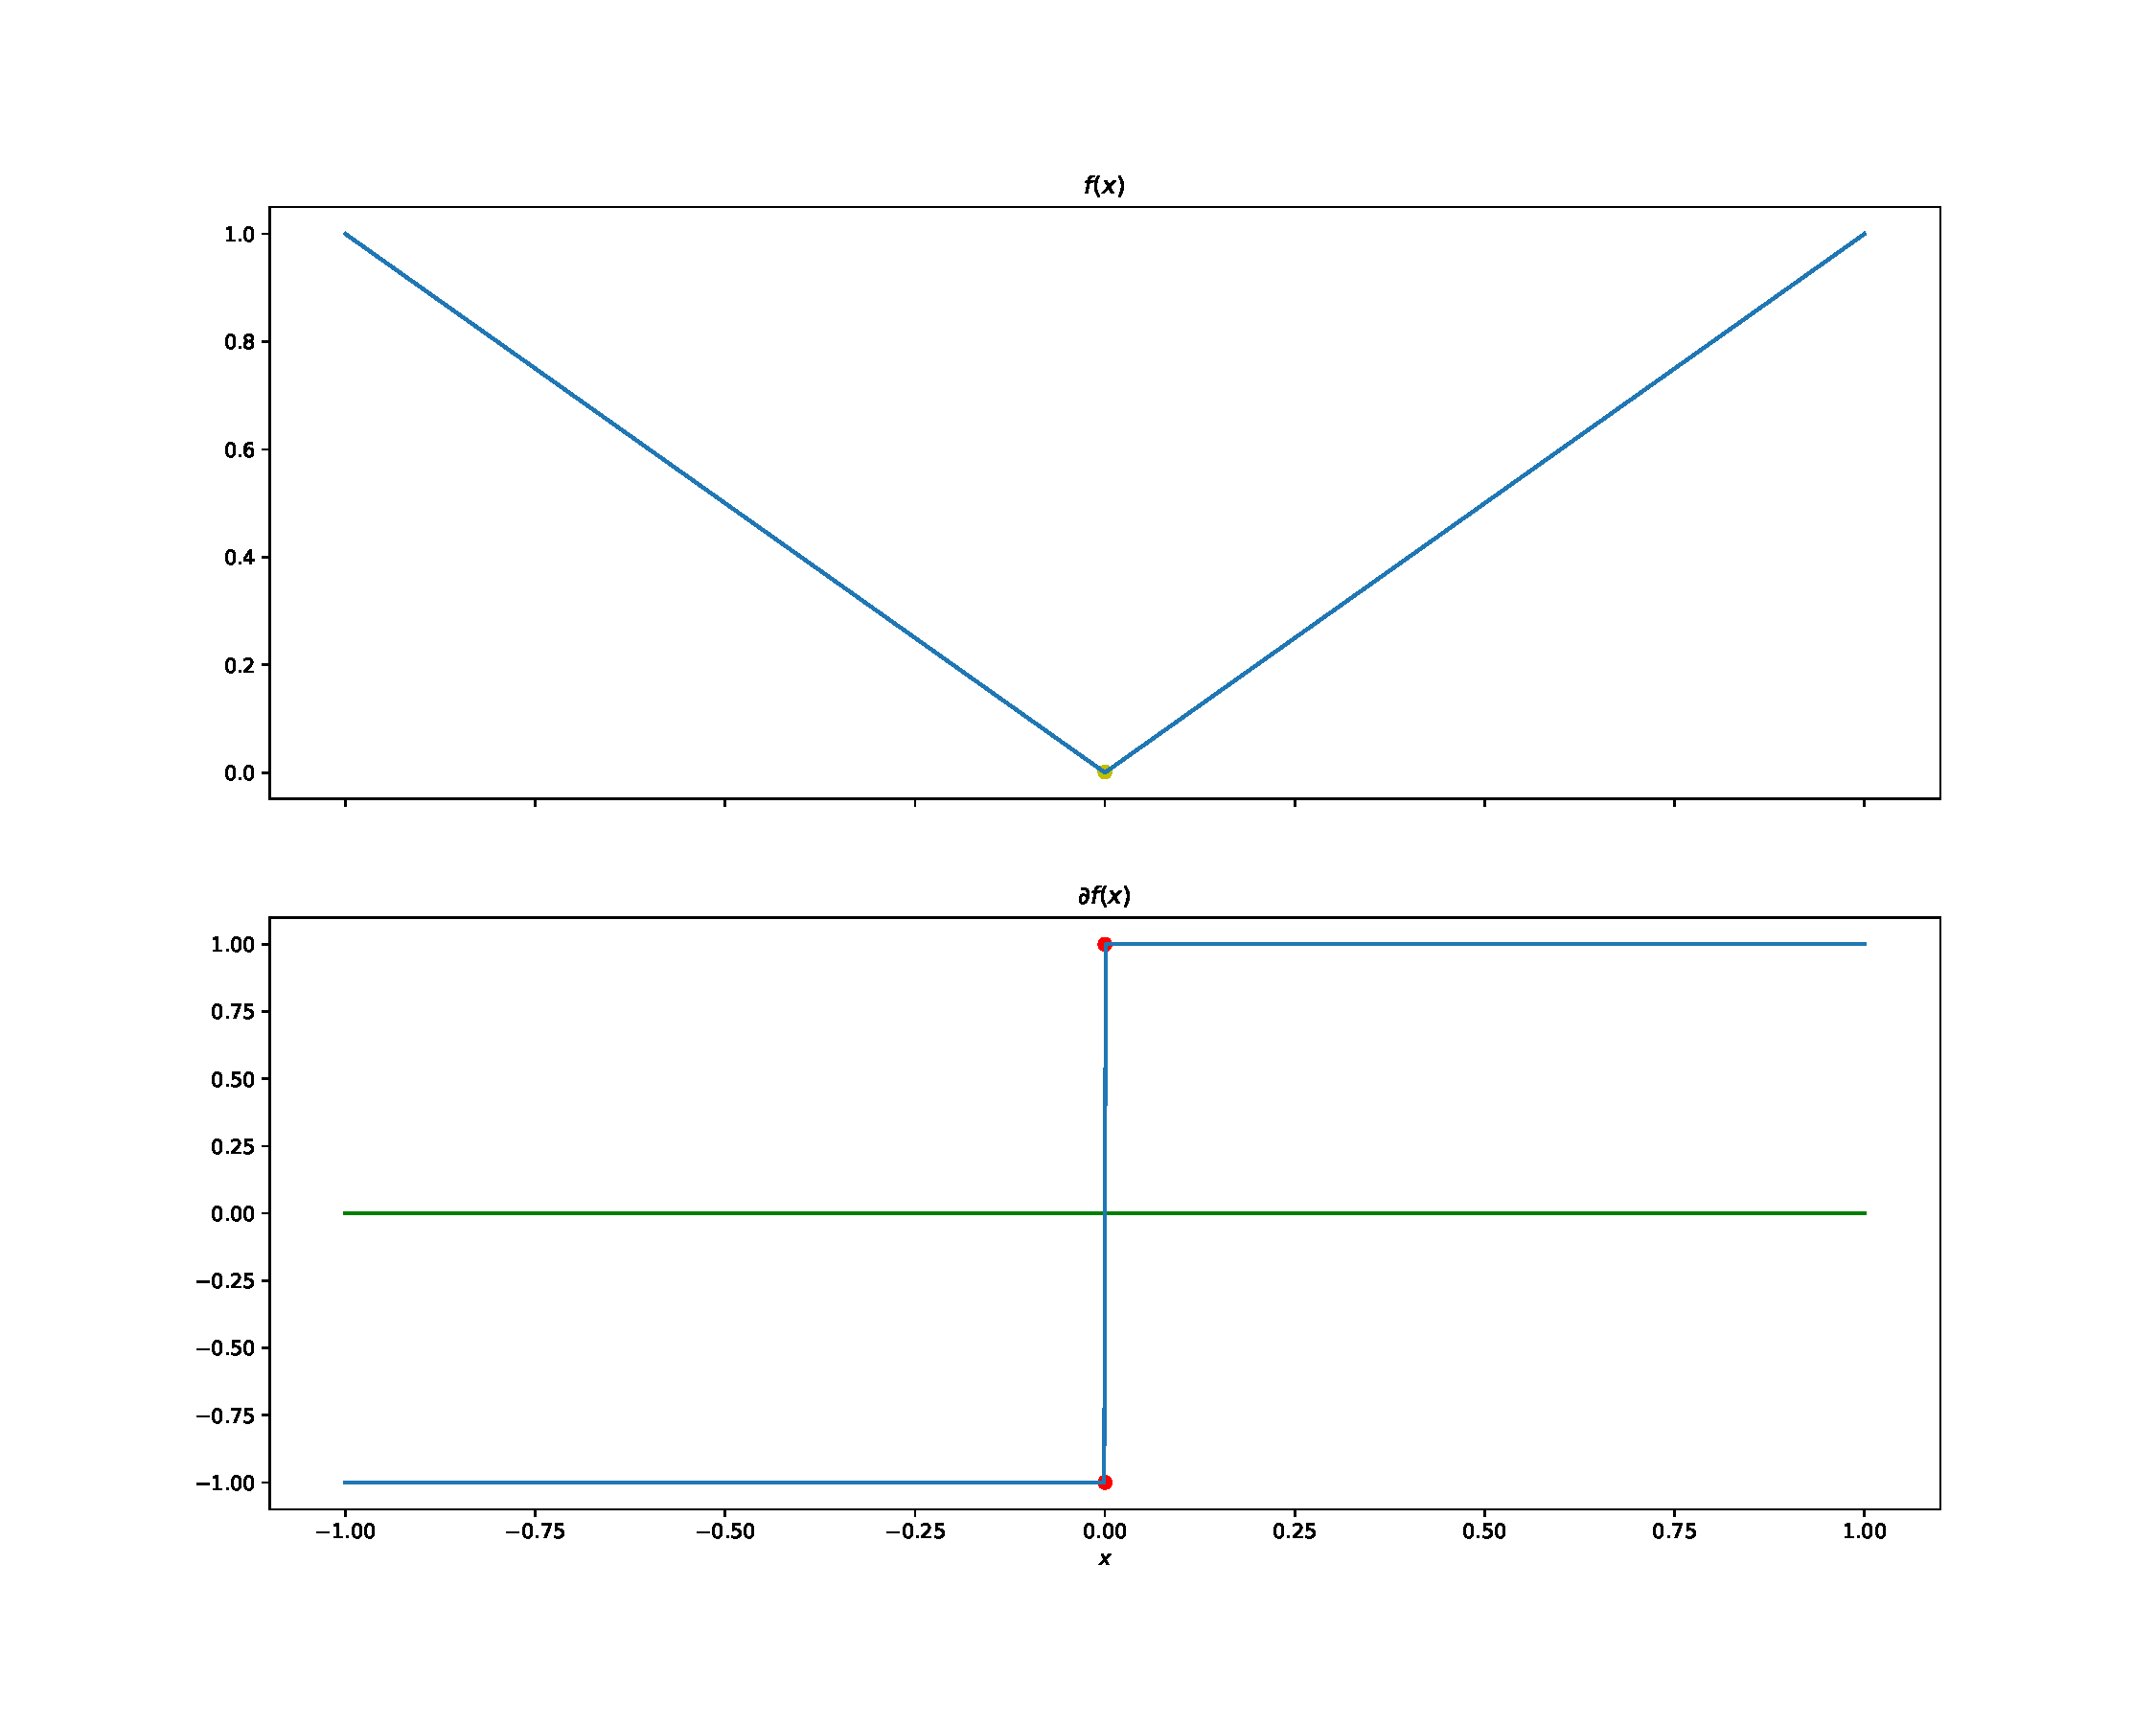
\includegraphics[width=\textwidth]{ejemplo1_mae.pdf}
    \caption{Absolute value function (top) and its corresponding subgradient (bottom). The green line represents the $0$ constant function. The blue dot is the point that is not differentiable and the red dots mark the interval of the corresponding subdifferential.}
    \label{fig:abs_loss}
\end{figure}
Using the formulation of~\eqref{eq:subproblem_lambda}, the training error corresponding to the absolute value loss is
\begin{equation}
    \label{eq:opt_abs}
    \argmin_{\lambda \in [0, 1]} \mathcal{J}(\lambda) = \sum_{i=1}^{\npertask} \abs{\lambda c_i + d_i}.
\end{equation}
Observe that in each term of the sum the subdifferential is 
\begin{align*}
    \partial \abs{\lambda c_i + d_i} = 
    \begin{cases}
        -\abs{c_i} &, \lambda c_i + d_i  < 0 \\
        [-\abs{c_i}, \abs{c_i}] &, \lambda c_i + d_i  = 0 \\
        \abs{c_i} &, \lambda c_i + d_i  > 0 \\
    \end{cases} 
\end{align*}
The elbows are obtained using the values $\frac{-d_i}{c_i}$, that can be clipped and sorted to get ${\lambda}_{(1)} < \ldots < {\lambda}_{(m)}$.
In~\citet[Proposition 2]{RuizAD21} we present a result to get the optimal $\lambda^*$.
\begin{prop}[Optimal $\lambda^*$ with absolute value loss]\label{prop:abs_neurocom2020}
    In problem~\eqref{eq:opt_abs} $\lambda^*=0$ is optimal iff
    \begin{equation}\nonumber
        - \sum_{j: \lambda_{(j)} < 0} \abs{c_{j}} + \sum_{j: \lambda_{(j)} > 0} \abs{c_{j}} < 0.
        \end{equation}
    If this condition does not hold, $\lambda^* \in (0,1)$ is optimal iff $\lambda^*$ is a feasible elbow, that is, $0 \leq \lambda^* = \lambda_{(k)} \leq 1$ for some $k=1, \dotsc, \npertask$, and
    \begin{equation}\label{sol_abs_e}
    - \sum_{j: \lambda_{(j)} < \lambda_{(k)}} \abs{c_{j}} + \sum_{j: \lambda_{(j)} > \lambda_{(k)}} \abs{c_{j}} \in \left[ -  \abs{c_{k}},  \abs{c_{k}}  \right] .
    \end{equation}
    If none of the previous conditions hold, then $\lambda^*=1$ is optimal.
\end{prop}
\begin{figure}[t!]
    \centering
    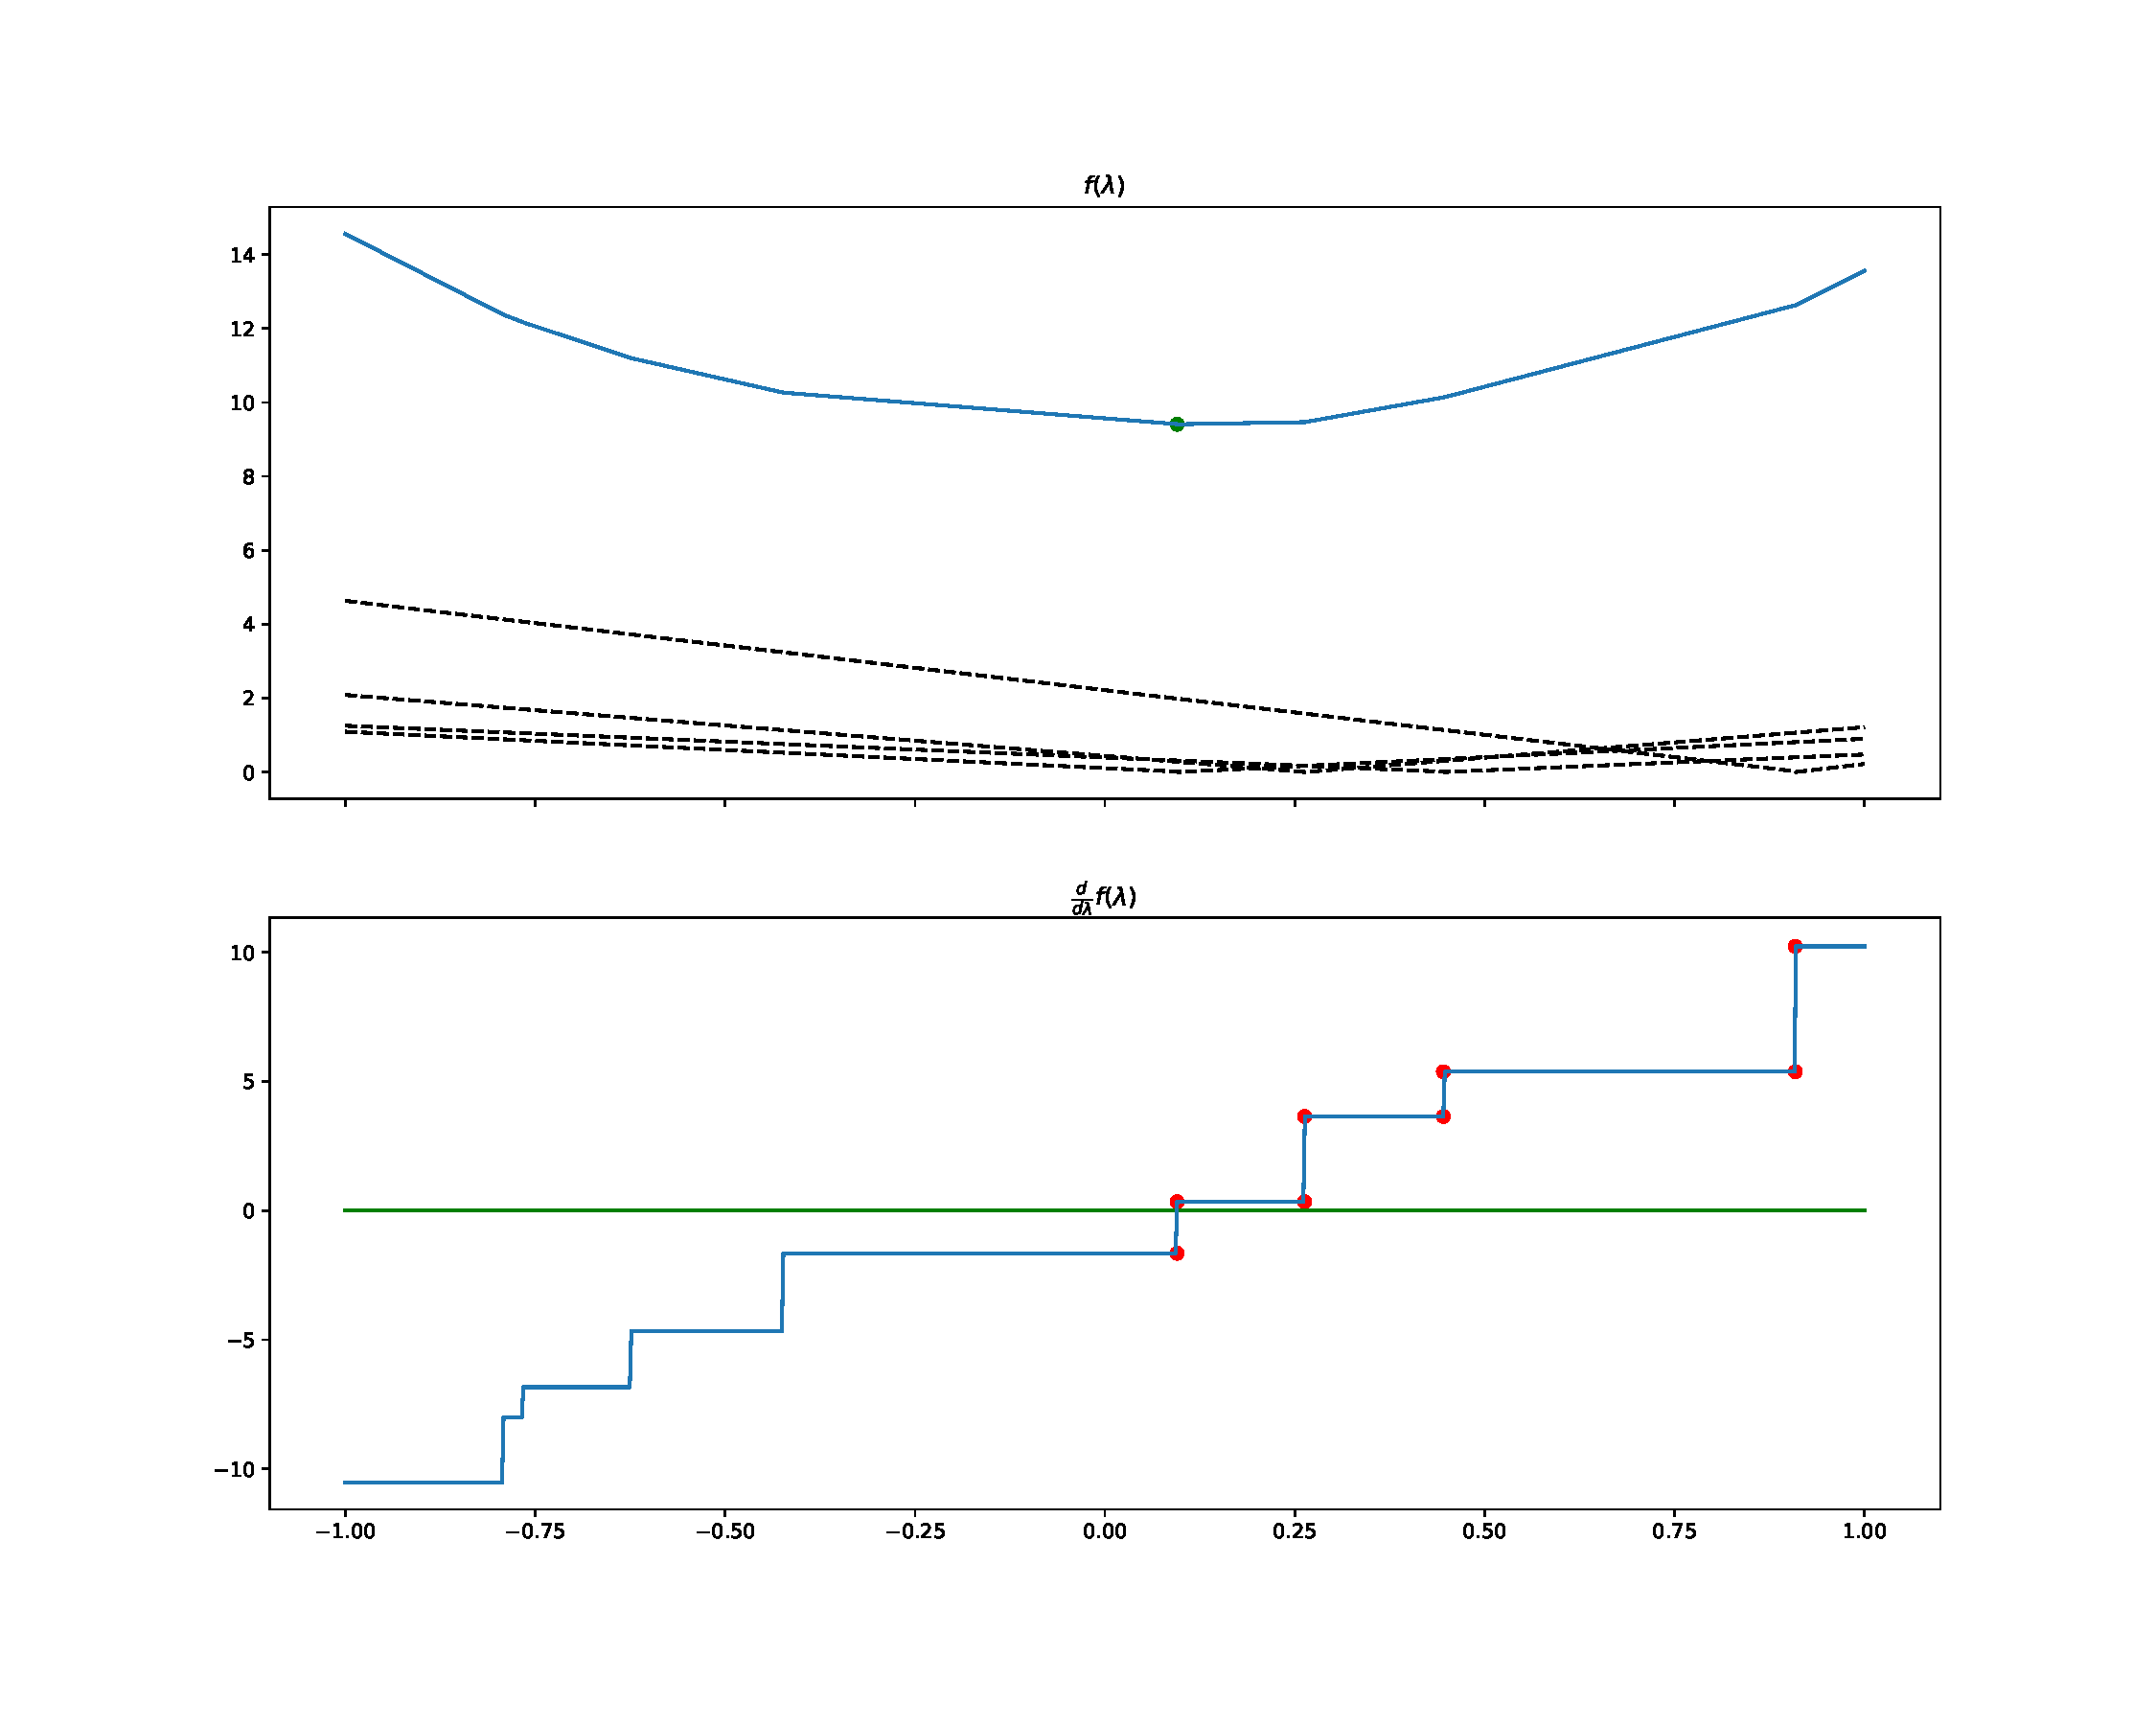
\includegraphics[width=\textwidth]{ejemplo2_mae.pdf}
    \caption{Error using absolute loss function (top) and its corresponding subgradient (bottom). The green line represents the $0$ constant function. The green dot is the point minimizing the error, and whose corresponding subgradient contains the value $0$.}
    \label{fig:abs_error}
\end{figure}

\subsection{Hinge loss}
\begin{figure}[t!]
    \centering
    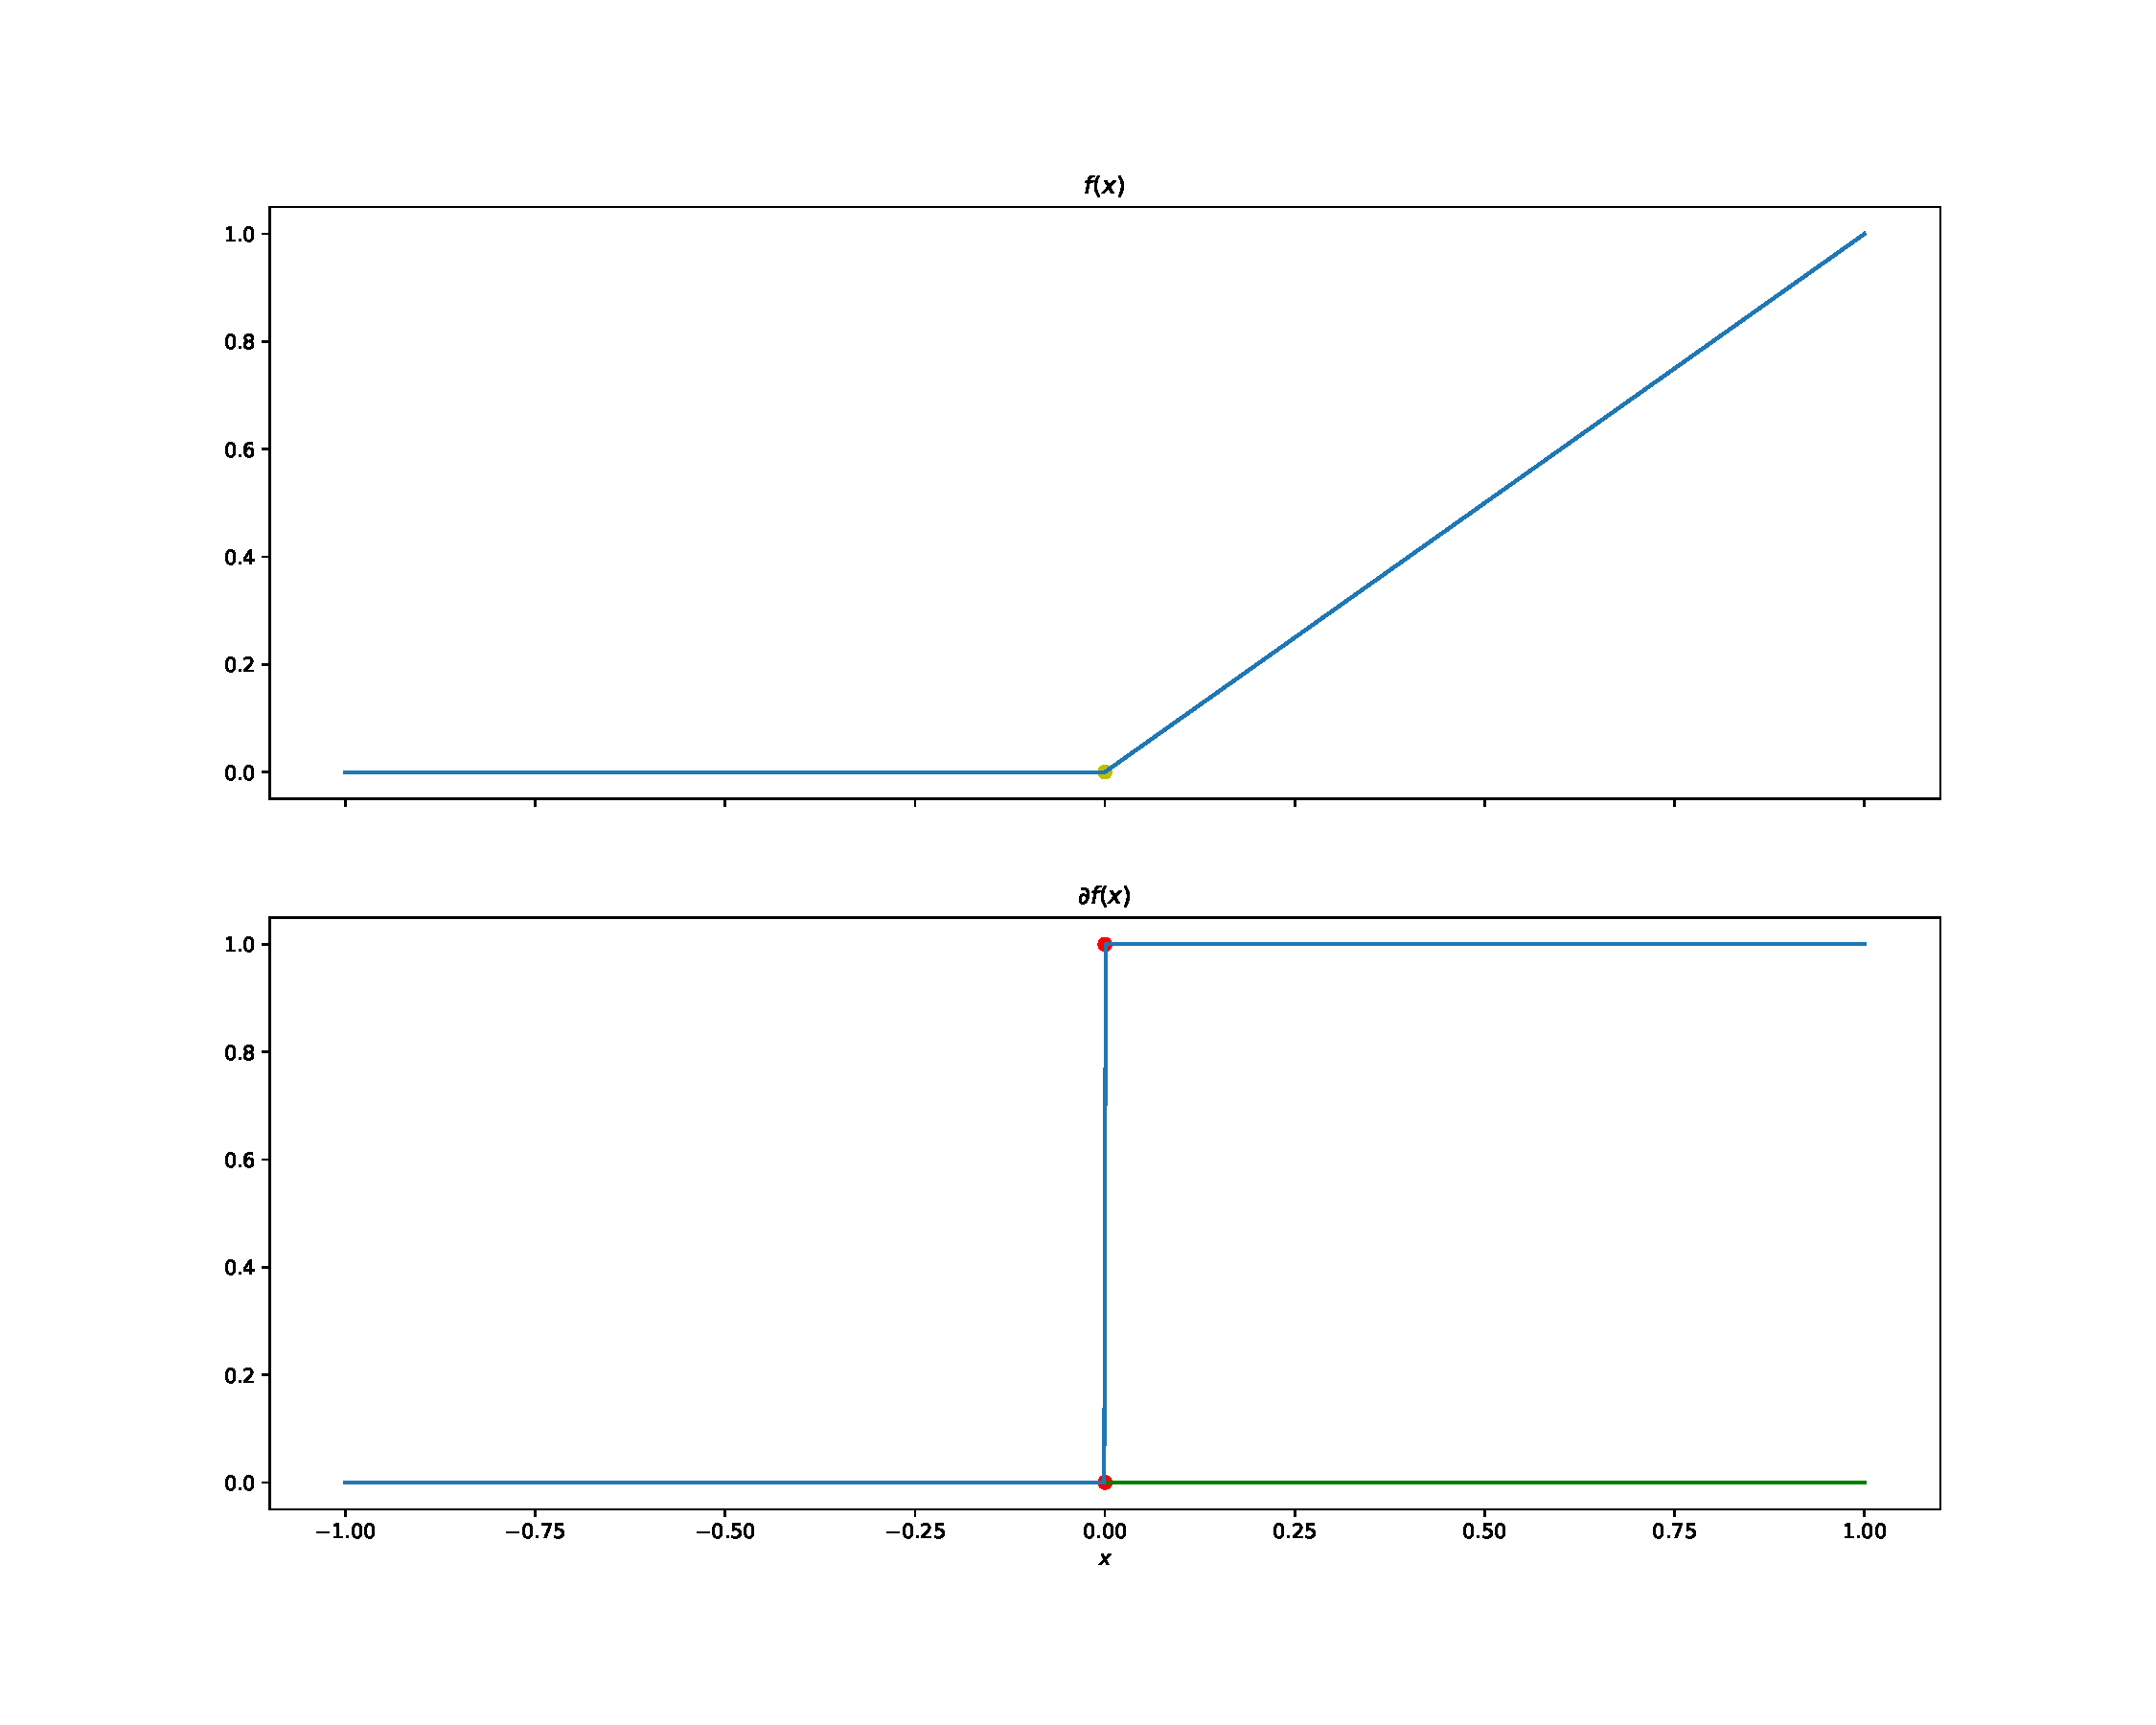
\includegraphics[width=\textwidth]{ejemplo1_hinge.pdf}
    \caption{Positive part function (top) and its corresponding subgradient (bottom). The green line represents the $0$ constant function. The blue dot is the point that is not differentiable and the red dots mark the interval of the corresponding subdifferential.}
    \label{fig:hinge_loss}
\end{figure}
Using the formulation of~\eqref{eq:subproblem_lambda}, the training error corresponding to the hinge loss is
\begin{equation}
    \label{eq:opt_hinge_l1}
    \argmin_{\lambda \in [0, 1]} \mathcal{J}(\lambda) = \sum_{i=1}^{\npertask} \pospart{\lambda c_i + d_i}.
\end{equation}
Observe that in each term of the sum the subdifferential is 
\begin{align*}
    \partial \left[\lambda c_i + d_i \right]_+ = 
    \begin{cases}
        0 &, \lambda c_i + d_i  < 0 \\
        [\min(0, c_i), \max(0, c_i)] &, \lambda c_i + d_i  = 0 \\
        c_i &, \lambda c_i + d_i  > 0 \\
    \end{cases} \; .
\end{align*}
That is, the elbows are related to the values $\frac{-d_i}{c_i}$, that can be clipped and sorted to obtain the elbows ${\lambda}_{(1)} < \ldots < {\lambda}_{(m)}$.
In~\citet[Proposition 2]{RuizAD21} we present a result to get the optimal $\lambda^*$.
\begin{prop}[Optimal $\lambda^*$ with hinge loss]\label{prop:hinge_neurocom2020}
    In~\eqref{eq:opt_hinge_l1}, $\lambda^*=0$ is optimal iff
    \begin{equation}\label{eq:sol_hinge_0}
        -\sum_{j: \lambda_{(j)}<0} \max(0, c_{(j)}) - \sum_{\lambda_{(j)}>0} \min(0, c_{(j)}) \leq 0 .
        \end{equation}
        If this condition does not hold, a value $\lambda^* \in (0, 1)$ is optimal for problem~\eqref{eq:opt_hinge_l1} iff $\lambda^* \in \set{0, 1}$ or $\lambda^*$ is a feasible elbow, that is, $0 \leq \lambda^* = \lambda_{(k)} \leq 1$ for some $k=1, \dotsc, \npertask$, and
    \begin{equation}\label{eq:sol_hinge}
        -\sum_{j: \lambda_{(j)}< \lambda_{(k)}} \max(0, c_{(j)}) - \sum_{j: \lambda_{(j)}>  \lambda_{(k)}} \min(0, c_{(j)}) \in \left[\min(0, c_{(k)}), \max(0, c_{(k)}) \right] .
    \end{equation}
    If none of the previous conditions hold, then $\lambda^*=1$ is optimal.
\end{prop}
\begin{figure}[t!]
    \centering
    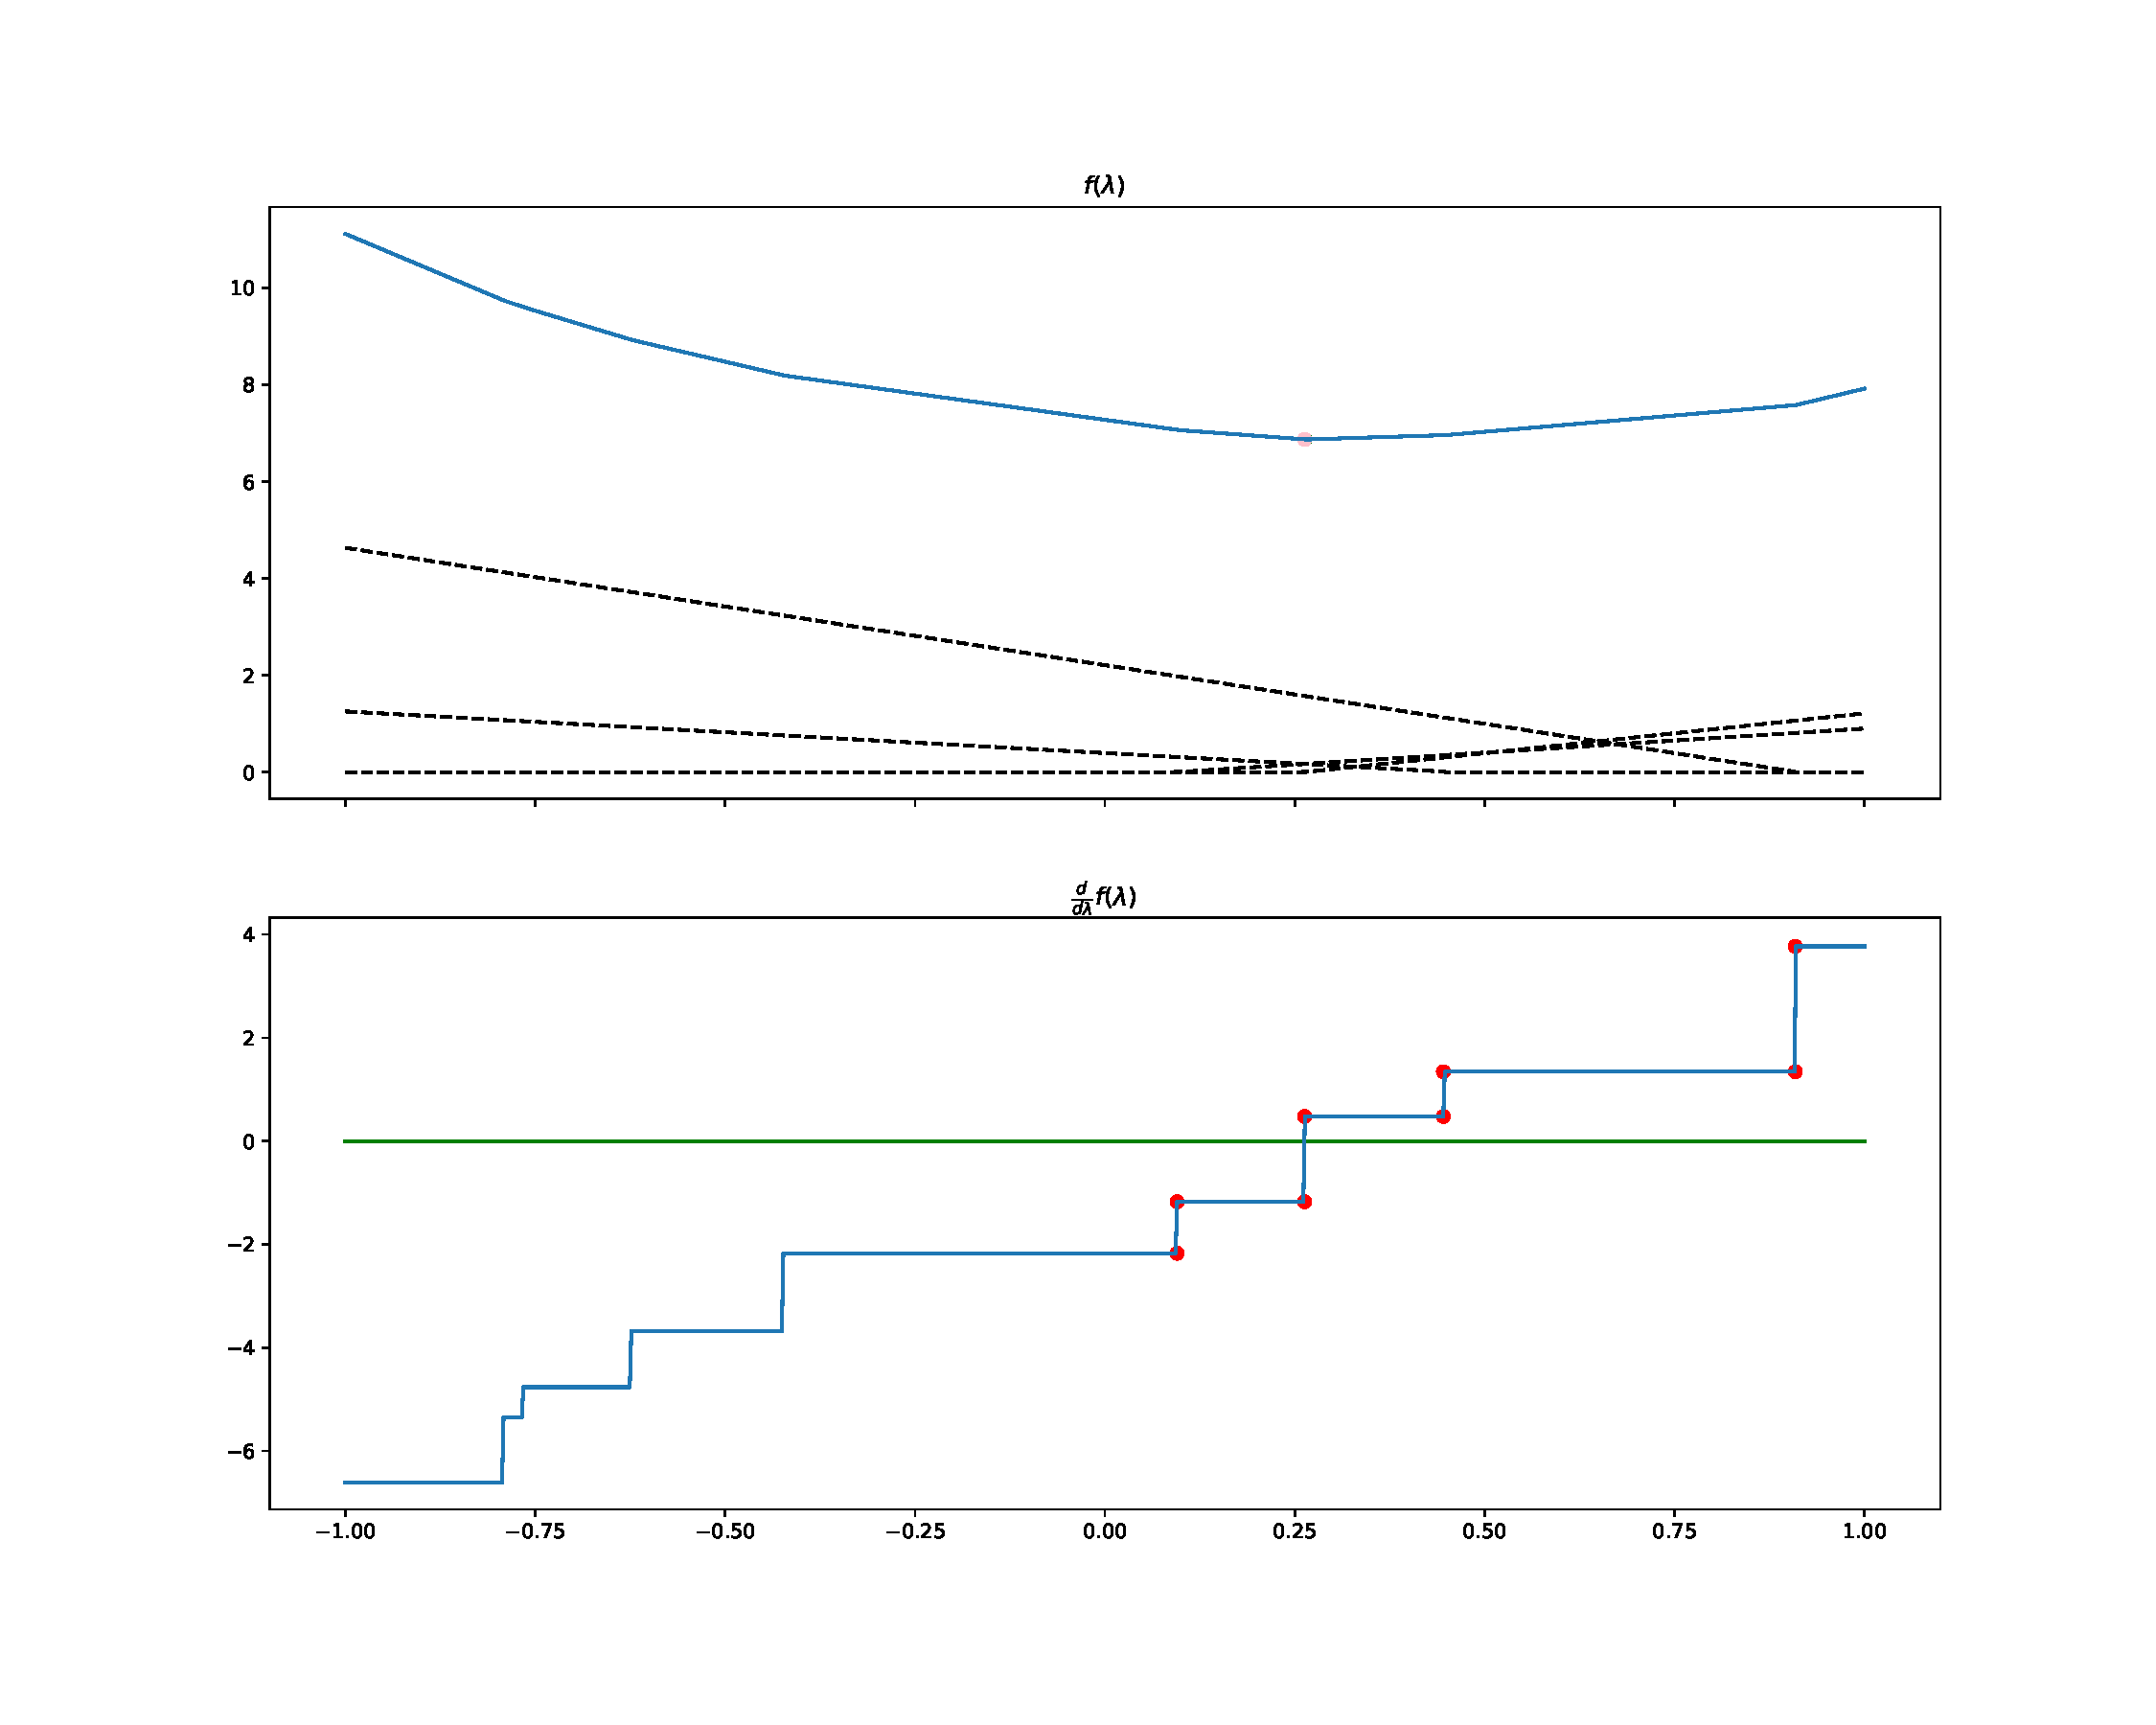
\includegraphics[width=\textwidth]{ejemplo2_hinge.pdf}
    \caption{Error using hinge loss function (top) and its corresponding subgradient (bottom). The green line represents the $0$ constant function. The green dot is the point minimizing the error, and whose corresponding subgradient contains the value $0$.}
    \label{fig:hinge_error}
\end{figure}

\subsection{Squared hinge loss}
Using the formulation of~\eqref{eq:subproblem_lambda}, the training error corresponding to the hinge loss is
\begin{equation}
    \label{eq:opt_hinge_l2}
    \argmin_{\lambda \in [0, 1]} \mathcal{J}(\lambda) = \sum_{i=1}^{\npertask} \pospart{\lambda c_i + d_i}^2.
\end{equation}
In each term of the sum the subdifferential is 
\begin{align*}
    \partial \left[\lambda c_i + d_i \right]_+^2 = 
    \begin{cases}
        0 &, \lambda c_i + d_i  \leq 0 \\
        2 c_i (\lambda c_i + d_i) &, \lambda c_i + d_i  > 0 \\
    \end{cases} \; .
\end{align*}
The elbows are again related to the values $\frac{-d_i}{c_i}$, that can be clipped and sorted to obtain the elbows ${\lambda}_{(1)} < \ldots < {\lambda}_{(m)}$.
In~\citet[Proposition 2]{RuizAD21} we give a result to get the optimal $\lambda^*$ when using the squared hinge loss.
\begin{prop}[Optimal $\lambda^*$ with squared hinge loss]\label{prop:sqhinge_neurocom2020}
    In~\eqref{eq:opt_hinge_l2},
    $\lambda^*=0$ is optimal iff 
    \begin{equation}\nonumber
         - \frac{\sum_{j: \lambda_{j} < 0} \max(0, c_{j}) d_{j} + \sum_{j: \lambda_{j} > 0} \min(0, c_{j}) d_{j}}{\sum_{j: \lambda_{j} < 0} \max(0, c_{j})^2 + \sum_{j: \lambda_{j} > 0} \min(0, c_{j})^2} < 0.
       \end{equation}
    If this condition does not hold, 
    consider the extended sorted list of feasible elbows $\lambda_{(p-1)} = 0 \leq \lambda_{(p)} \leq \ldots, \lambda_{(q)} \leq \lambda_{(q+1)}=1$, with $1 \leq p, q \leq m$, and
    define for $k=p-1, \ldots,  q$ $\widehat{\lambda}_k$ as %
\begin{equation}\label{sol_hinge_2}
 \widehat{\lambda}_k = - \frac{\sum_{j: \lambda_{(j)} < \lambda_{(k)}} \max(0, c_{j}) d_{j} + \sum_{j: \lambda_{(j)} > \lambda_{(k)}} \min(0, c_{j}) d_{j}}{\sum_{j: \lambda_{(j)} < \lambda_{(k)}} \max(0, c_{j})^2 + \sum_{j: \lambda_{(j)} > \lambda_{(k)}} \min(0, c_{j})^2} .
\end{equation}
%
Then, if $\lambda_k \leq \widehat{\lambda}_k \leq  \lambda_{k+1}$ for some $\widehat{\lambda}_k$, then $\lambda^* = \widehat{\lambda}_k$ is optimal.
Finally, if none of the previous conditions holds, \eqref{eq:opt_hinge_l2} has a minimum at $\lambda^* = 1$.
\end{prop}


\section{Convex Multi-Task Learning with Neural Networks}
The convex MTL formulation is easily applicable and interpretable, so it has good properties for kernel models, but also for a broader class of learning models.
Neural networks, in particular deep ones, have had a massive success in multiple applications. Moreover, they are very flexible models whose architecture can be adapted to fulfill different goals. In this section we show how to use our convex formulation for MTL with neural networks.

%
In Chapter~\ref{Chapter3} we have reviewed the taxonomy for MTL methods, and the approaches can be broadly grouped in three categories: feature-based, parameter-based and combination-based. 
We also show in Subsection~\ref{subsec:deep_mtl} some of the most famous approaches to MTL with neural networks. Most of these approaches can fit in the feature-based category, where the shared layers are fully or partially shared to obtain a latent representation that is useful for all tasks, as shown in Figure~\ref{fig:hardsharing_nn}; see for example~\cite{Caruana97, MisraSGH16,RuderBAS17}. Some approaches rely also on a parameter-based view, where the parameters of each task-specific network are regularized together so that they are close in some sense, see~\cite{Long015a, YangH17a}.
However, to the best of my knowledge, the first purely combination-based approach to MTL with neural networks is presented in~\cite{RuizAD22_hais}, where we use a convex combination of neural networks.

\begin{figure}[t!]
    \centering
    \begin{tikzpicture}
 
        % Input Layer
        \foreach \i in {1,...,\inputnum}
        {
            \node[circle, 
                minimum size = 6mm,
                fill=orange!30] (Input-\i) at (0,-\i) {};
        }
         
        
        % Hidden Layer 1
        \foreach \i in {1,...,\hiddennumhs}
        {
            \node[circle, 
                minimum size = 6mm,
                fill=teal!50,
                yshift=(\hiddennumhs-\inputnum)*5 mm
            ] (Hidden1-\i) at (2.5,-\i) {};
        }
        
        % Hidden Layer 2
        \foreach \i in {1,...,\hiddennumhs}
        {
            \node[circle, 
                minimum size = 6mm,
                fill=teal!50,
                yshift=(\hiddennumhs-\inputnum)*5 mm
            ] (Hidden2-\i) at (5,-\i) {};
        }
         
        % Output Layer
        \foreach \i in {1,...,\outputnum}
        {
            \node[circle, 
                minimum size = 6mm,
                fill=purple!50,
                yshift=(\outputnum-\inputnum)*5 mm
            ] (Output-\i) at (7.5,-\i) {};
        }
         
        % Connect neurons In-Hidden
        \foreach \i in {1,...,\inputnum}
        {
            \foreach \j in {1,...,\hiddennumhs}
            {
                \draw[->, shorten >=1pt, red!80!black, densely dashdotted] (Input-\i) -- (Hidden1-\j);   
            }
        }

        % Connect neurons Hidden-Hidden
        \foreach \i in {1,...,\hiddennumhs}
        {
            \foreach \j in {1,...,\hiddennumhs}
            {
                \draw[->, shorten >=1pt, red!80!black, densely dashdotted] (Hidden1-\i) -- (Hidden2-\j);   
            }
        }
         
        % Connect neurons Hidden-Out
        \foreach \i in {1,...,\hiddennumhs}
        {
            \foreach \j in {1}
            {
                \draw[->, shorten >=1pt, blue!80!black, dashed] (Hidden2-\i) -- (Output-\j);
            }
        }

        \foreach \i in {1,...,\hiddennumhs}
        {
            \foreach \j in {2,...,\outputnum}
            {
                \draw[->, shorten >=1pt] (Hidden2-\i) -- (Output-\j);
            }
        }
         
        % Inputs
        \foreach \i in {1,...,\inputnum}
        {            
            \draw[<-, shorten <=1pt] (Input-\i) -- ++(-1,0)
                node[left]{};
        }
         
        % Outputs
        \foreach \i in {1,...,\outputnum}
        {            
            \draw[->, shorten <=1pt] (Output-\i) -- ++(1,0)
                node[right]{$h_{\i}(\fv{x})$};
        }
         
    \end{tikzpicture}
    \caption{\emph{Hard Sharing} Neural Network for two tasks and a two-dimensional input. Assuming a sample belonging to task $1$ is used, the updated shared weights are represented in red, and in blue the updated specific weights. 
    The input neurons are shown in yellow, the hidden ones in cyan and the output ones in magenta.
    }
    \label{fig:hardsharing_nn}
\end{figure}

\subsection{Model Definition}
Using the formulation of~\eqref{eq:convexmtl_general}, we use neural networks to the model the common part 
$$ g(x_i^r; w, \Theta) = w^\intercal f(x_i^r; \Theta) + b,$$
and task-specific parts
$$ g_r(x_i^r; w_r, \Theta_r) =  w_r^\intercal f_r(x_i^r; \Theta_r) + b_r.$$
Here $\Theta$ and $\Theta_r$ are the sets of hidden weights, $w$, $w_r$ are the output weights of the common and specific networks, respectively, and $b$ and $b_r$ the output biases.
Observe that the feature transformations $ f(x_i^r; \Theta)$ and $f_r(x_i^r; \Theta_r)$ are not fixed like $\phi(x_i^r)$ and $\phi_r(x_i^r)$ in the kernel methods, instead, here, they are automatically learned in the training process.
The full MTL models are then
\begin{equation}
    \label{eq:convexmtl_nn}
    \begin{aligned}
        h_r(x_i^r)
       = \lambda \lbrace w^\intercal f(x_i^r; \Theta) + b \rbrace + (1 - \lambda) \lbrace w_r^\intercal f_r(x_i^r; \Theta_r) + b_r \rbrace.
    \end{aligned}    
\end{equation}

This formulation offers multiple combinations since we can model each common or independent function using different architectures for $f(\cdot; \Theta)$ or $f_r(\cdot; \Theta_r)$.
%
For example, we can use a network with a larger number of parameters for the common part, since it will be fed with more data, and simpler networks for the task-specific parts.
%
Even different types of neural networks, such as fully connected and convolutional, can be combined depending on the characteristics of each task.
% Connection with LUPI
This combination of neural networks can also be interpreted as an implementation of the LUPI paradigm~\citep{VapnikI15a} shown in Subsection~\ref{subsec:ch3_lupi}, i.e., the common network captures the privileged information for each of the tasks, since it can learn from more sources.
%

%
\subsection{Training Procedure}
The regularized risk corresponding to the convex MTL neural networks is
\begin{equation}
    \label{eq:regrisk_convex_nn}
    \begin{aligned}
        \risk_{\bsample} = \sum_{r=1}^\ntasks \sum_{i=1}^{m} \lossf(h_r(x_i^r), y_i^r) + \frac{\mu}{2} \left( \norm{w}^2 + \sum_{r=1}^\ntasks \norm{w_r}^2 + \Omega(\Theta) + \Omega(\Theta_r)\right) .
    \end{aligned}
\end{equation}
Here, $h_r$ is defined as in equation~\eqref{eq:convexmtl_nn}, and $\Omega(\Theta)$ and $\Omega(\Theta_r)$ represents the $L_2$ regularization of the set of hidden weights of the common and specific networks, respectively.
Given a loss function $\lossf(\hat{y}, y)$ and a pair $(x_i^t, y_i^t)$ from task $t$, we use the chain rule to compute the gradient of the loss function with respect to some parameters $\mathcal{P}$:
\begin{equation}\label{eq:gradient_p}
    \nabla_\mathcal{P} \lossf(h_t(x_i^t), y_i^t) = 
    \frac{\partial}{\partial \hat{y}_i^t} \lossf(\hat{y}_i^t, y_i^t) \vert_{\hat{y}_i^t = h_t(x_i^t)} \nabla_\mathcal{P} h_t(x_i^t) .
\end{equation}
Recall that we are using the formulation 
$$h_t(x_i^t)
= \lambda \lbrace w^\intercal f(x_i^t; \Theta) + b \rbrace + (1 - \lambda) \lbrace w_t^\intercal f_t(x_i^t; \Theta_t) + b_t \rbrace, $$
where we make a distinction between output weights $w, w_t$ and hidden parameters $\Theta, \Theta_t$.
Then, the corresponding gradients of $h_t$ needed to compute the loss gradients are
\begin{equation}\label{eq:gradients_losses} 
    \begin{aligned}       
        &\nabla_{w} h_t(x_i^t)  
        = \lambda \lbrace f(x_i^t, \Theta) \rbrace ,
        &&\nabla_{\Theta} h_t(x_i^t)  
        = \lambda \lbrace w^\intercal \nabla_\Theta f(x_i^t, \Theta)\rbrace ; \\
        &\nabla_{w_t} h_t(x_i^t)  
        = (1 - \lambda) \lbrace f_t(x_i^t, \Theta) \rbrace ,
        &&\nabla_{\Theta_t} h_t(x_i^t)  
        = (1 - \lambda) \lbrace  w^\intercal \nabla_{\Theta_t} f_t(x_i^t, \Theta_t)\rbrace ; \\
        &\nabla_{w_r} h_t(x_i^t)  
        =  0 , 
        &&\nabla_{\Theta_r} h_t(x_i^t)  
        =  0 , \text{ for } r \neq t .\\
    \end{aligned}    
\end{equation}
Putting all together, the gradient of the loss with respect to $w$, for example, is 
$$  \nabla_w \lossf(h_t(x_i^t), y_i^t)  =\lossf(\hat{y}_i^t, y_i^t) \vert_{\hat{y}_i^t = h_t(x_i^t)} \lambda \lbrace f(x_i^t, \Theta), \rbrace $$
and the same for the rest of parameters.
%
Observe that the convex combination information is transferred in the back-propagation, the loss gradients with respect to common parameters are scaled by $\lambda$, while those of the task-specific parameters are scaled by $(1 - \lambda)$.
%
Moreover, the regularization of each set of parameters, i.e., $\set{w}, \Theta$ and $\set{w_r}, \Theta_r$, is done independently, so their gradients can be computed in the standard way.
%
During the back propagation procedure, we only update the parameters that have been used in the forward pass, with possibly different learning rates for each network. 
That is, given an example $(x_i^t, y_i^t)$, when using vanilla \acrshort{sgd} the update rules for the common network parameters would be
\begin{equation}\label{eq:convexmtl_nn_commonupdate}
    \begin{aligned}
        w^{\tau + 1} &\gets w^\tau + \eta \left[  \frac{\partial}{\partial \hat{y}_i^t}  \lossf(\hat{y}_i^t, y_i^t) \vert_{\hat{y}_i^t = h_t(x_i^t)} \lambda \lbrace f(x_i^t, \Theta) \rbrace + \mu w^\tau \right], \\
        \Theta^{\tau + 1} &\gets \Theta^\tau + \eta \left[ \frac{\partial}{\partial \hat{y}_i^t}  \lossf(\hat{y}_i^t, y_i^t) \vert_{\hat{y}_i^t = h_t(x_i^t)}  \lambda \lbrace w^\intercal \nabla_\Theta f(x_i^t, \Theta)\rbrace + \mu \lbrace \nabla_\Theta \Omega( \Theta)  \rbrace \right];
    \end{aligned}
\end{equation}
while the update rules for $t$-th task network parameters would be
\begin{equation}\label{eq:convexmtl_nn_specificupdate}
    \begin{aligned}
        w_t^{\tau + 1} &\gets w_t^\tau + \eta_t \left[  \frac{\partial}{\partial \hat{y}_i^t}  \lossf(\hat{y}_i^t, y_i^t) \vert_{\hat{y}_i^t = h_t(x_i^t)} (1 - \lambda) \lbrace f(x_i^t, \Theta) \rbrace + \mu w_t^\tau \right], \\
        \Theta_t^{\tau + 1} &\gets \Theta_t^\tau + \eta_t \left[ \frac{\partial}{\partial \hat{y}_i^t}  \lossf(\hat{y}_i^t, y_i^t) \vert_{\hat{y}_i^t = h_t(x_i^t)}  (1 - \lambda) \lbrace w^\intercal \nabla_{\Theta_t} f(x_i^t, \Theta_t)\rbrace + \mu \lbrace \nabla_{\Theta_t} \Omega( \Theta_t) \rbrace \right];
    \end{aligned}
\end{equation}
and the parameters from the rest of task-specific network are not updated.
%
That is, no specific algorithm has to be developed for training the convex MTL NN. In~\eqref{eq:convexmtl_nn_commonupdate} and~\eqref{eq:convexmtl_nn_specificupdate} we have shown the update rules for vanilla SGD, but any other algorithm, e.g., Adam, can be used scaling properly the loss gradients.

\begin{figure}[t!]
    \centering
    \begin{tikzpicture}

        % Input Layer
        \foreach \i in {1,...,\inputnum}
        {
            \node[circle, 
                minimum size = \minnodesize,
                fill=orange!30] (Input_common-\i) at (0,-\i- \hiddennum) {};
        }

        \node[circle, 
            minimum size = \minnodesize,
            fill=purple!30] (Pred1) at (8,-1.2 * \hiddennum) {};

        \node[circle, 
        minimum size = \minnodesize,
        fill=purple!30] (Pred2) at (8,-2.2 * \hiddennum) {};

        \draw[->, shorten <=1pt] (Pred1) -- ++(1,0)
            node[right]{$h_1(\fv{x})$};

        \draw[->, shorten <=1pt] (Pred2) -- ++(1,0)
        node[right]{$h_2(\fv{x})$};

        %%%%%%%%%%%%%%%%%%%% Specific NN 1 %%%%%%%%%%%%%%%%%%%%%%%%%%
    %     % Input Layer
    % \foreach \i in {1,...,\inputnum}
    % {
    %     \node[circle, 
    %         minimum size = \minnodesize,
    %         fill=orange!30] (Input_sp1-\i) at (0,-\i) {};
    % }
     
    
    % Hidden Layer 1
    \foreach \i in {1,...,\hiddennum}
    {
        \node[circle, 
            minimum size = \minnodesize,
            fill=teal!50,
            yshift=(\hiddennum-\inputnum)*5 mm
        ] (Hidden1_sp1-\i) at (2,-\i) {};
    }
    
    % Hidden Layer 2
    \foreach \i in {1,...,\hiddennum}
    {
        \node[circle, 
            minimum size = \minnodesize,
            fill=teal!50,
            yshift=(\hiddennum-\inputnum)*5 mm
        ] (Hidden2_sp1-\i) at (4,-\i) {};
    }
     
    % Output Layer
    \foreach \i in {1,...,1}
    {
        \node[circle, 
            minimum size = \minnodesize,
            fill=black!50,
            yshift=(1-\inputnum)*5 mm
        ] (Output_sp1-\i) at (6,-\i) {$g_1(\fv{x})$};
    }
     
    % Connect neurons In-Hidden
    \foreach \i in {1,...,\inputnum}
    {
        \foreach \j in {1,...,\hiddennum}
        {
            \draw[->, shorten >=1pt,blue!80!black, dashed] (Input_common-\i) -- (Hidden1_sp1-\j);   
        }
    }


    % Connect neurons Hidden-Hidden
    \foreach \i in {1,...,\hiddennum}
    {
        \foreach \j in {1,...,\hiddennum}
        {
            \draw[->, shorten >=1pt,blue!80!black, dashed] (Hidden1_sp1-\i) -- (Hidden2_sp1-\j);   
        }
    }
     
    % Connect neurons Hidden-Out
    \foreach \i in {1,...,\hiddennum}
    {
        \foreach \j in {1,...,1}
        {
            \draw[->, shorten >=1pt,blue!80!black, dashed] (Hidden2_sp1-\i) -- (Output_sp1-\j);
        }
    }
     
    % % Inputs
    % \foreach \i in {1,...,\inputnum}
    % {            
    %     \draw[<-, shorten <=1pt] (Input_sp1-\i) -- ++(-1,0)
    %         node[left]{$x_{\i}$};
    % }
     
    % Outputs
    % \foreach \i in {1,...,1}
    % {            
    %     \draw[->, shorten <=1pt] (Output_sp1-\i) -- ++(2,0)
    %         node[right]{$g_1(x)$};
    % }

    \draw[->, ultra thick] (Output_sp1-1) -- (Pred1) node [midway, fill=white] {$1 - \lambda$};

    
    
    \draw[thick]     ($(Hidden1_sp1-1.north west)+(-0.5,0.15)$) rectangle ($(Output_sp1-1.south east)+(0.3,-0.45)$);
    
    
    %%%%%%%%%%%%%%%%%% Common NN %%%%%%%%%%%%%%%%%%%%%%%%%%%%%%%%%%%

    
     
    
    % Hidden Layer 1
    \foreach \i in {1,...,\hiddennum}
    {
        \node[circle, 
            minimum size = \minnodesize,
            fill=teal!50,
            yshift=(\hiddennum-\inputnum)*5 mm
        ] (Hidden1_common-\i) at (2,-\i- \hiddennum) {};
    }
    
    % Hidden Layer 2
    \foreach \i in {1,...,\hiddennum}
    {
        \node[circle, 
            minimum size = \minnodesize,
            fill=teal!50,
            yshift=(\hiddennum-\inputnum)*5 mm
        ] (Hidden2_common-\i) at (4,-\i- \hiddennum) {};
    }
     
    % Output Layer
    \foreach \i in {1,...,1}
    {
        \node[circle, 
            minimum size = \minnodesize,
            fill=black!50,
            yshift=(1-\inputnum)*5 mm
        ] (Output_common-\i) at (6,-\i- \hiddennum) {$g(\fv{x})$};
    }
     
    % Connect neurons In-Hidden
    \foreach \i in {1,...,\inputnum}
    {
        \foreach \j in {1,...,\hiddennum}
        {
            \draw[->, shorten >=1pt,red!80!black, densely dashdotted] (Input_common-\i) -- (Hidden1_common-\j);   
        }
    }

    % Connect neurons In-Hidden
    \foreach \i in {1,...,\hiddennum}
    {
        \foreach \j in {1,...,\hiddennum}
        {
            \draw[->, shorten >=1pt,red!80!black, densely dashdotted] (Hidden1_common-\i) -- (Hidden2_common-\j);   
        }
    }
     
    % Connect neurons Hidden-Out
    \foreach \i in {1,...,\hiddennum}
    {
        \foreach \j in {1,...,1}
        {
            \draw[->, shorten >=1pt,red!80!black, densely dashdotted] (Hidden2_common-\i) -- (Output_common-\j);
        }
    }
     
    % Inputs
    \foreach \i in {1,...,\inputnum}
    {            
        \draw[<-, shorten <=1pt] (Input_common-\i) -- ++(-1,0)
            node[left]{};
    }
     
    % % Outputs
    % \foreach \i in {1,...,1}
    % {            
    %     \draw[->, shorten <=1pt] (Output_common-\i) -- ++(2,0)
    %         node[right]{$g(x)$};
    % }

    \draw[->, ultra thick] (Output_common-1) -- (Pred1) node [midway, fill=white] {$\lambda$};
    \draw[->, ultra thick] (Output_common-1) -- (Pred2) node [midway, fill=white] {$\lambda$};


    \draw[thick,blue,dotted]     ($(Hidden1_common-1.north west)+(-0.5,0.15)$) rectangle ($(Output_common-1.south east)+(0.3,-0.45)$);

    %%%%%%%%%%%%%%%%%%%% Specific NN 2 %%%%%%%%%%%%%%%%%%%%%%%%%%
        % % Input Layer
        % \foreach \i in {1,...,\inputnum}
        % {
        %     \node[circle, 
        %         minimum size = \minnodesize,
        %         fill=orange!30] (Input_sp2-\i) at (0,-\i- 2*\hiddennum) {};
        % }
         
        
        % Hidden Layer 1
        \foreach \i in {1,...,\hiddennum}
        {
            \node[circle, 
                minimum size = \minnodesize,
                fill=teal!50,
                yshift=(\hiddennum-\inputnum)*5 mm
            ] (Hidden1_sp2-\i) at (2,-\i- 2*\hiddennum) {};
        }
        
        % Hidden Layer 2
        \foreach \i in {1,...,\hiddennum}
        {
            \node[circle, 
                minimum size = \minnodesize,
                fill=teal!50,
                yshift=(\hiddennum-\inputnum)*5 mm
            ] (Hidden2_sp2-\i) at (4,-\i- 2*\hiddennum) {};
        }
         
        % Output Layer
        \foreach \i in {1,...,1}
        {
            \node[circle, 
                minimum size = \minnodesize,
                fill=black!50,
                yshift=(1-\inputnum)*5 mm
            ] (Output_sp2-\i) at (6,-\i- 2*\hiddennum) {$g_2(\fv{x})$};
        }
         
        % Connect neurons In-Hidden
        \foreach \i in {1,...,\inputnum}
        {
            \foreach \j in {1,...,\hiddennum}
            {
                \draw[->, shorten >=1pt] (Input_common-\i) -- (Hidden1_sp2-\j);   
            }
        }
    
        % Connect neurons In-Hidden
        \foreach \i in {1,...,\hiddennum}
        {
            \foreach \j in {1,...,\hiddennum}
            {
                \draw[->, shorten >=1pt] (Hidden1_sp2-\i) -- (Hidden2_sp2-\j);   
            }
        }
         
        % Connect neurons Hidden-Out
        \foreach \i in {1,...,\hiddennum}
        {
            \foreach \j in {1,...,1}
            {
                \draw[->, shorten >=1pt] (Hidden2_sp2-\i) -- (Output_sp2-\j);
            }
        }
         
        % % Inputs
        % \foreach \i in {1,...,\inputnum}
        % {            
        %     \draw[<-, shorten <=1pt] (Input_sp2-\i) -- ++(-1,0)
        %         node[left]{$x_{\i}$};
        % }
         
        % Outputs
        % \foreach \i in {1,...,1}
        % {            
        %     \draw[->, shorten <=1pt] (Output_sp2-\i) -- ++(2,0)
        %         node[right]{$g_2(x)$};
        % }

        \draw  [->, ultra thick] (Output_sp2-1) -- (Pred2) node [midway, fill=white] {$1 - \lambda$};
         
        \draw[thick]     ($(Hidden1_sp2-1.north west)+(-0.5,0.15)$) rectangle ($(Output_sp2-1.south east)+(0.3,-0.45)$);

    \end{tikzpicture}
    \caption[Convex \acrshort{mtl} neural network for two tasks and a two-dimensional input.]{Convex \acrshort{mtl} neural network for two tasks and a two-dimensional input.
    Assuming a sample belonging to task $1$ is used, the updated shared weights are represented in red, and in blue the updated specific weights. 
    Specific networks are framed in black boxes and the common one in a blue box.
    The input neurons are shown in yellow, the hidden ones in cyan (except those in grey), and the output ones in magenta. 
    We use the grey color for hidden neurons containing the intermediate functions that will be combined for the final output: $g_1(\fv{x})$, $g_2(\fv{x})$ and $g(\fv{x})$.
    The thick lines are the hyperparameters $\lambda$ and $1-\lambda$ of the convex combination. 
	}
    \label{fig:convexmtl_nn}
\end{figure}



% In Figure~\ref{fig:convexmtl_nn}, a Convex MTL NN is shown. % in the gradient update step.
%     In particular, the updated shared weights are represented in red, and in blue the updated specific weights. 
%     Specific networks are framed in black boxes and the common one in a blue box.
%     The input neurons are shown in yellow, the hidden ones in cyan (except those in grey), and the output ones in magenta. 
%     We use the grey color for hidden neurons containing the intermediate functions that will be combined for the final output: $g_1(\fv{x})$, $g_2(\fv{x})$ and $g(\fv{x})$.
%     The thick lines are the hyperparameters $\lambda$ and $1-\lambda$ of the convex combination.

\subsection{Implementation Details}
% Task-batches of minibatches
% Automatic differentiation

Our implementation of the convex MTL neural network is based on \texttt{PyTorch}~\citep{PyTorch}.
Although we include the gradients expressions in equation~\eqref{eq:gradients_losses}, the \texttt{PyTorch} package implements automatic differentiation, so the gradients are not explicitly implemented.
Instead, we implement each network, common or specific, using (possibly different) \texttt{PyTorch} modules.
In the forward pass of the network, the output for an example $x_i^r$ from task $r$ is computed using a pass of the common module and the corresponding specific module, combining both passes with the convex formulation to obtain the final output $h_r(x_i^r)$.
In the training phase, in which minibatches are used, the full minibatch is passed through the common model, but the minibatch is task-partitioned, where each partition is passed through its corresponding specific module.
By doing this, when using examples from the $r$-th task only the parameters corresponding to common module and its corresponding specific one are updated.
Moreover, as mentioned above, with the adequate forward pass, the \texttt{PyTorch} package automatically computes the scaled gradients in the training phase.

{In Algorithm~\ref{alg:forward} we show the pseudo-code of the forward pass of the convex MTL neural network. Here, $g$ and $g_1, \ldots, g_\ntasks$ are the common and task-specific modules, whose outputs are combined. We do not show the backward pass because we rely on PyTorch automatic differentiation.}

\begin{algorithm}[!t]
    \DontPrintSemicolon
      
      \KwInput{$X_\text{mb}, t_\text{mb}$ \tcp*{Minibatch data and task labels}}
      \KwOutput{$f$ \tcp*{Forward pass for the minibatch}}
      \KwData{$\lambda$ \tcp*{Parameter of convex combination}}
      \KwData{$g; g_1, \ldots, g_\ntasks$ \tcp*{Modules of the common and specific networks}}      
      \For{$x_i, t_i \in(X_\text{mb}, t_\text{mb}) $}    
            { 
                $f_i \gets \lambda g(x_i) + (1 - \lambda) g_{t_i}(x_i)$   \tcp*{Convex combination}

            }
    \caption{Forward pass for Convex MTL neural network.}
    \label{alg:forward}
\end{algorithm}


\section{Experiments}

\section{Conclusions}\label{sec-conclusions-3}

In this chapter, we have\dots
